\documentclass[12pt]{article}
\usepackage{units}
\usepackage{tikz}
\usepackage{lettrine}
\usepackage{hyperref}
\usepackage{polski}
\usepackage[utf8]{inputenc}
\usepackage{acro}
\usepackage{booktabs}
\usepackage{graphicx}
\usepackage{siunitx}
\usepackage{makeidx}
\makeindex

\hypersetup{
	colorlinks=true,
	linkcolor=green,
	filecolor=magenta,      
	urlcolor=cyan,
}

\urlstyle{same}

\newcommand{\doi}[1]{doi: \href{htts://doi.org/#1}{#1}}
\newcommand{\ra}[1]{\renewcommand{\arraystretch}{#1}}
\newcommand{\specialcell}[2][c]{%
  \begin{tabular}[#1]{@{}c@{}}#2\end{tabular}}

\title{Komentarz do ,,Stanowiska Komitetu Nauk Geologicznych Polskiej Akademii Nauk w debacie klimatycznej''}

\author{@doskonaleszare}

\begin{document}
\maketitle

Ujednolicona i~lekko przeredagowana wersja blognotek do stanowiska KNG PAN opublikowanych pierwotnie na blogu ,,Doskonale Szare''\footnote{\url{https://doskonaleszare.github.io}.}.

\subsection*{Streszczenie}

Dzięki geologii wiemy, że klimat naszej planety wielokrotnie się zmieniał w~bliższej i~odległej przeszłości. Zmiany te były powodowane różnymi czynnikami: wahaniami aktywności słonecznej, periodycznymi zmianami orbity ziemskiej, erupcjami wulkanicznymi, a~także zmianami zawartości gazów cieplarnianych w~atmosferze. Badania paleoklimatyczne (w~tym modelowanie klimatu Ziemi w~odległej przeszłości) umożliwiają nam stawianie i~weryfikowanie hipotez dotyczących przyczyn tych zmian klimatu, jednak ze względu na niepewności dotyczące rekonstrukcji stanu środowiska sprzed tysięcy czy milionów lat, nie zawsze jest możliwe ustalenie ponad wszelką wątpliwość jak i~dlaczego zmieniał się klimat w~przeszłości geologicznej planety.

Dla odmiany, obecne zmiany klimatu możemy obserwować bezpośrednio dzięki globalnej sieci stacji meteorologicznych, radiosond, radarów, satelitów, samolotów, statków, boi,~pływaków i~dronów oceanograficznych. Obserwacje i~pomiary, w~połączeniu z~teoretycznym opisem procesów zachodzących w~systemie klimatycznym, umożliwiają nam zdiagnozowanie przyczyn globalnego ocieplenia zachodzącego od ponad 100 lat, i~wykazanie ponad wszelką wątpliwość, że odpowiedzialna jest za nie emisja gazów cieplarnianych, przede wszystkim spalanie węgla, ropy i~gazu. Tempo współczesnej, antropogenicznej zmiany klimatu jest pod wieloma względami bezprecedensowe w~skali przynajmniej kilku milionów lat.

Nie jest to tylko opinia klimatologów czy fizyków atmosfery; z diagnozą taką zgadzają się również badacze zajmujący się badaniem klimatu w~odległej przeszłości, a~także instytucje i~organizacje zrzeszające geologów i~innych specjalistów z~zakresu nauk o~Ziemi. Powszechna akceptacja antropogenicznych przyczyn globalnego ocieplenia jest widoczna chociażby w~treści współczesnych podręczników, również do geologii.

Na tym tle stanowisko Komitetu Nauk Geologicznych Polskiej Akademii Nauk szokuje nie tylko treścią, ale i~formą, w~tym selektywnym doborem źródeł i~skromną bibliografią. Jasne jest, że jego autorzy nie znają się na większości zagadnień o~których napisali, nie konsultowali się ze specjalistami, ani nie robili systematycznego przeglądu literatury. W~wielu przypadkach pisali ,,z głowy'', w~oparciu o~analizę znalezionych w~internecie wykresów metodą ,,na oko'', a~tam gdzie cytowali jakąś literaturę naukową, to często bez zrozumienia, albo były to prace dawno już zdezaktualizowane.

Nie będę spekulować nad przyczynami takiego stanu rzeczy, i~nie mam złudzeń że bez wymiany pokoleniowej nie ma co liczyć na głębszą refleksję członków Komitetu. Na szczęście dzisiaj widać wyraźniej niż kiedykolwiek, jak bardzo oderwane od świata nauki jest część środowiska polskich geologów, i~pozostaje mi mieć nadzieję, że opinia KNG szybko zostanie zapomniana jako wstydliwy relikt ostatniego bastionu denializmu klimatycznego.
\newpage

\subsection*{Rola geologii w~badaniach nad klimatem}

\begin{quotation}
	Dziesięć lat temu Komitet Nauk Geologicznych PAN (KNG PAN) przedstawił swoje stanowisko w kwestii ocieplenia klimatu wskazując, że zmiany klimatu w geologicznej skali czasu są zjawiskiem naturalnym, a ocieplenie obserwowane współcześnie należy powściągliwie interpretować jako (wyłączny bądź dominujący) skutek działalności człowieka. Wobec rosnącej intensywności aktualnej debaty klimatycznej, czujemy się w obowiązku ponownie zająć stanowisko w tej sprawie.\footnote{
	Stanowisko KNG PAN (wersja datowana na 9 grudnia 2019 r., \url{http://www.kngpan.agh.edu.pl/wp-content/uploads/Stanowisko-KNG\_klimat\_2019.pdf}) jest podzielone na fragmenty, ale cytowane w~całości. Rysunki oznaczone jako ,,fig.~1'', ,,fig.~3'' i~,,fig.~6'' również pochodzą z~tekstu KNG wraz z podpisami. Śródtytuły pochodzą ode mnie, z~wyjątkiem tych wewnątrz cytatowanych fragmentów opinii KNG.}
\end{quotation}

Zacznę od sprostowania chronologii: pierwsze stanowisko powstało po posiedzeniu Komitetu z dnia 11 listopada 2008 roku, na którym jego członkowie poczuli się w obowiązku podzielić się z opinią publiczną swoimi przemyśleniami. Pierwotna wersja tego dokumentu zawierała wiele rażących błędów, o których pisałem na moim świeżo wtedy założonym blog\footnote{\url{https://web.archive.org/web/20170311195435/http://doskonaleszare.blox.pl/2009/02/Ignorancja-Komitetu-Nauk-Geologicznych-PAN.html}}; wersja ostateczna, datowana na 12 lutego i opublikowana 2 marca 2009, niektóre z tych błędów poprawiła, choć w dalszym ciągu zawierało ono sformułowania sprzeczne z ustaleniami nauki odnośnie obserwowanych zmian klimatu i ich przyczyn.

\begin{quotation}
	Ocieplenie klimatu w skali globalnej, od około 150 lat dokumentowane jest przez naukę bezpośrednimi pomiarami temperatury oraz obserwacjami tak spektakularnych procesów jak zmniejszanie zasięgu lodu morskiego czy recesje lodowców górskich i polarnych. Jest ono skorelowane z zapoczątkowanym około 150 lat temu szybkim rozwojem przemysłu epoki industrialnej, który opiera się na paliwach kopalnych: węglu, ropie, gazie ziemnym. Ich spalanie powoduje emisję do atmosfery CO$_2$, który jest jednym z tzw.~gazów cieplarnianych. Wzrost zawartości CO$_2$ w atmosferze, monitorowany bezpośrednimi pomiarami od 1955 roku (krzywa Keelinga), zdecydowana większość badaczy uważa za przyczynę ocieplenia klimatu. Ten pogląd, upowszechniany przez media, wywołuje głębokie zaniepokojenie opinii publicznej, co skłania rządy wielu krajów do podejmowania gwałtownych i kosztownych działań dla zahamowania i zaprzestania emisji CO$_2$ do atmosfery. W niniejszym opracowaniu proponujemy spojrzenie na relacje CO$_2$--temperatura w geologicznej skali czasu dla lepszego zrozumienia ich wzajemnego związku przyczynowo-skutkowego.
\end{quotation}

To dobrze, że członkowie Komitetu Nauk Geologicznych zauważyli, że \emph{zdecydowana większość badaczy} uważa antropogeniczne emisje gazów cieplarnianych za przyczynę globalnego ocieplenia, choć jednocześnie wydają się być zaskoczeni tym, że media upowszechniają wiedzę odnośnie wniosków tychże badaczy, że zaniepokojenie naukowców --- w tym członków akademii nauk krajów takich jak Stany Zjednoczone, Niemcy, Chin, Kanady, Wielkiej Brytanii, Australii, a nawet Polski --- powoduje zaniepokojenie opinii publicznej, i że politycy podejmują działania oparte o ustalenia nauki (choć można polemizować, czy te działania zasługują na określenie ,,gwałtowne'').

Oczywiście, geologiczne spojrzenie na relacje pomiędzy dwutlenkiem węgla a temperaturą ma swoje miejsce w klimatologii --- IPCC na przykład poświęciło temu zagadnieniu cały rozdział piątego raportu opublikowanego w 2013\footnote{\url{https://www.ipcc.ch/report/ar5/wg1/information-from-paleoclimate-archives/}}, temat ten podejmowały również inne organizacje zrzeszające geologów (np. brytyjskie Geological Society\footnote{\url{https://www.geolsoc.org.uk/climatechange}} --- ale treść stanowiska KNG PAN po raz kolejny pokazuje, że polscy naukowcy tej specjalności albo nie znają aktualnej literatury przedmiotu, albo nie potrafią jej poprawnie zinterpretować.

\begin{quotation}
	Argumenty z dziedziny geologii w debacie klimatycznej to informacje o stanie powierzchni Ziemi w przeszłości przedindustrialnej, gdy decydowały o tym stanie na pewno czynniki naturalne. Geologia dostarcza przede wszystkim pewnej wiedzy, że naczelną cechą klimatu Ziemi w całej jej historii jest zmienność. Zmiany zachodzą w nakładających się cyklach o różnej długości trwania --- od kilkunastu lat do dziesiątków milionów lat --- rządzonych splotem wielu czynników pozaziemskich i ziemskich. Zmiany klimatu są wymuszane także przez procesy aperiodyczne, wynikające z ewolucji Słońca, zmienności  koncentracji gazów szklarniowych w atmosferze, kumulacji działalności wulkanicznej czy impaktów asteroidów. Klimatotwórcze współzależności między nimi nie zostały jeszcze w pełni rozpoznane.
\end{quotation}

Geologia dostarcza nam więc wiedzy dotyczącej tego, że klimat nie zmienia się \emph{sam z siebie}, ale że za jego zmiany odpowiadają wymienione czynniki. Jednym z tych czynników jest, jak zauważyli geolodzy z KNG, zawartość gazów cieplarnianych w atmosferze, na którą to zawartość ludzkość ma obecnie wpływ, w odróżnieniu od działalności wulkanicznej, impaktów asteroidów i ewolucji Słońca.

Jest prawdą że w odniesieniu do odległej przeszłości nie rozpoznano wszystkich czynników, które powodowały te czy inne zmiany klimatu. Jest to nieuniknione, bo klimat Ziemi sprzed milionów lat możemy badać wyłącznie metodami pośrednimi, które zawsze obciążone będą dużymi niepewnościami. Zmianę klimatu zachodzącą \emph{obecnie} możemy natomiast obserwować \emph{bezpośrednio}, dzięki pomiarom dokonywanym w stacjach meteorologicznych, przez radiosondy, satelity, boje oceanograficzne, i wiele innych typów platform pomiarowych. Z tego też powodu więcej możemy powiedzieć o przyczynach i przebiegu \emph{obecnego} globalnego ocieplenia, niż np. globalnego ocieplenia na przełomie paleocenu i eocenu. I jak przewidziano teoretycznie już dawno temu\footnote{Arrhenius S.~(1896): ,,On the Influence of Carbonic Acid in the Air upon the Temperature of the Ground'', \doi{10.1086/121158}.}, i potwierdzono w późniejszych badaniach\footnote{Stott P., et al.~(2000): ,,External Control of 20th Century Temperature by Natural and Anthropogenic Forcings'', \doi{10.1126/science.290.5499.2133}.}, główną przyczyną jest działalność człowieka.

\newpage

\subsection*{Zmiany klimatu ciągu ostatnich 500 milionów lat}

\begin{quotation}
	\textbf{Zmienność temperatur w skali setek milionów lat (fanerozoik)}
	
	W interesującej nas kwestii związku koncentracji CO$_2$ w atmosferze z temperaturą na powierzchni Ziemi trzeba stwierdzić, że zapis geologiczny nie wskazuje na istnienie prostej zależności korelacyjnej między tymi dwiema zmiennymi. Dostępne informacje o cyklach najdłuższych --- w skali epok geologicznych --- wskazują, że najwyższe średnie temperatury (do 14\si{\celsius} wyższe od współczesnych) panowały na Ziemi ok.~480 mln lat temu: na granicy kambru i ordowiku, przed 270 mln lat --- w permie oraz ok.~80 mln lat temu: w późnej kredzie, najniższe zaś (parę stopni niższe od współczesnych) ok.~450 mln lat temu: w  ordowiku i przed ok. 25 000 lat (Fig.~1, 2). Poziom CO$_2$ spadł z kilku tysięcy ppm w kambrze (ok. 520 mln lat) do kilkuset ppm w karbonie (ok. 300 mln lat), następnie wzrósł do ponad 2000 ppm w mezozoiku i spadł ponownie do kilkuset ppm w neogenie (ostatnie 20 mln lat). W takiej skali widać korelację długotrwałych (dziesiątki mln lat) minimów temperaturowych z minimami poziomu CO$_2$ (karbon i neogen), ale już na przełomie jury i kredy temperatura spadła do poziomu dzisiejszego, podczas gdy poziom CO$_2$ był sześciokrotnie wyższy niż dziś. Taka sytuacja jest sprzeczna z paradygmatem efektu cieplarnianego. Podobny paradoks dotyczy zlodowacenia ordowickiego (Fig.~1) czy okresu holoceńskiego (Fig.~5 poniżej), kiedy poziom koncentracji CO$_2$ i metanu wzrasta, a temperatura spada, począwszy od ok.~7000 lat temu. Należy  więc dopuścić hipotezę o istnieniu innych czynników warunkujących klimat, które potrafiły stłumić efekt szklarniowy.

	Najciekawsze --- jako analog dla współczesności --- ocieplenie po okresie lodowcowym na początku permu przyszło wcześniej niż wyraźny wzrost CO$_2$ z końcem permu. Te obserwacje sugerują, że w cyklach najdłuższych nie ma prostej zależności przyczynowo-skutkowej między poziomem CO$_2$ w atmosferze a temperaturą na powierzchni Ziemi.
\end{quotation}

Ten krótki fragment ilustruje większość związanych ze stanowiskiem KNG PAN problemów. Autorzy zaczynają od zbudowania chochoła: choć dosłownie akapit wcześniej wymieniali \emph{różne} czynniki które miały wpływ na klimat, teraz nagle odkrywają, że zapis geologiczny nie wskazuje na istnienie \emph{prostej} zależności korelacyjnej pomiędzy koncentracją CO$_2$ w atmosferze a temperaturą powierzchni Ziemi, oraz że należy dopuścić hipotezę \emph{innych} czynników warunkujących klimat.

\emph{No shit, Sherlock}. Nikt przecież nie kwestionuje, że na klimat wpływają różne czynniki. Być może geologom z PAN wydaje się, że istnienie \emph{różnych} czynników determinujących klimat w przeszłości geologicznej Ziemi jest sprzeczne z tym, że \emph{obecnie} klimat zmienia się głównie pod wpływem \emph{jednego}, dominującego czynnika. Jeśli tak uważają, to jest to wniosek błędny.

Drugim, być może większym nawet problemem jest to, w jaki sposób geolodzy z KNG PAN dobierają źródła. Można byłoby oczekiwać, że trzydziestu kilku zawodowych geologów będzie potrafiło w tak ważnym dokumencie skonstruować porządną bibliografię, a pojawiające się w stanowisku tezy będą podpierane odnośnikami do recenzowanych publikacji, prezentujących najnowsze ustalenia geologiczne i paleoklimatyczne. Nic z tych rzeczy: źródłem ,,fig.~1'' (poniżej) jest przysłowiowy ,,internet'', i pochodzi z pseudonaukowego bloga Watts Up With That.

\begin{figure}
	\centering	
	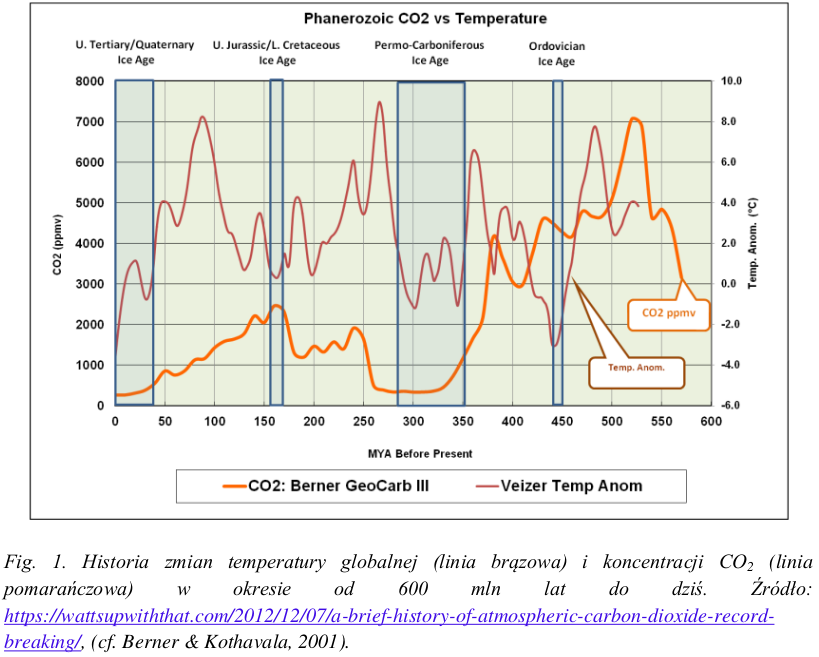
\includegraphics[width=.95\textwidth]{img/kng1.png};
\end{figure}

Cóż z tego, zapytacie, może i źródło kiepskie, ale wykres jest poprawny? Otóż właśnie nie bardzo.

Jeśli się przeklikacie przez bloga cytowanego przez KNG PAN, odkryjecie że źródłem autora wykresu jest kolejny, starszy wpis na tym samym blogu, ale dane użyte do jego narysowania dawno temu rozpłynęły się w czeluściach internetu. Nie jest to problemem w przypadku rekonstrukcji dwutlenku węgla w atmosferze\footnote{Berner R.~A., Kovathala Z.~(2001):~,,GEOCARB III: A revised model of atmospheric CO$_2$ over Phanerozoic time'', \doi{10.2475/ajs.301.2.182}.}, bo zostały one zarchiwizowane na serwerach NOAA\footnote{\url{https://www.ncdc.noaa.gov/paleo-search/study/5778}.}, jednak krzywa temperaturowa jest opracowaniem własnym autora bloga, opartym o kompilację danych izotopowych opublikowaną przez Jana Veizera w 1999 roku\footnote{Veizer J., et al.~(1999):~,,$^{87}$Sr/$^{86}$Sr, $\delta^{13}$C and $\delta^{18}$O evolution of Phanerozoic seawater", \doi{10.1016/S0009-2541(99)00081-9}.}.

Wykres prezentuje więc w \emph{najlepszym} razie stan wiedzy sprzed 20 lat. Co gorsza, użyte dane nie zostały rzetelnie przedstawione: choć wiadomo, że zależność amplitudy globalnego ocieplenia klimatu od zmiany zawartości dwutlenku węgla jest logarytmiczna, wykres przedstawia obie krzywe w liniowym układzie współrzędnych. Dodatkowo zostały one silnie wygładzone, i nie ma na wykresie niepewności związanych z rekonstruowanymi parametrami.

A te są spore. Rekonstrukcja temperatury pochodzi z badań skamielin (przede wszystkim małży), w których wykorzystano zależność frakcjonacji izotopowej $^{18}$O w cząsteczkach węglanu wapnia od temperatury. Metoda ta stosowana jest z powodzeniem do rekonstrukcji paleoklimatycznych z okresu plejstocenu, a nawet kenozoiku, jednak jej stosowanie do starszych okresów jest problematyczne, bo próbki pochodzące z odległej przeszłości zawierają sporo mniej $^{18}$O niż te powstałe stosunkowo niedawno.

\begin{figure}
	\centering
	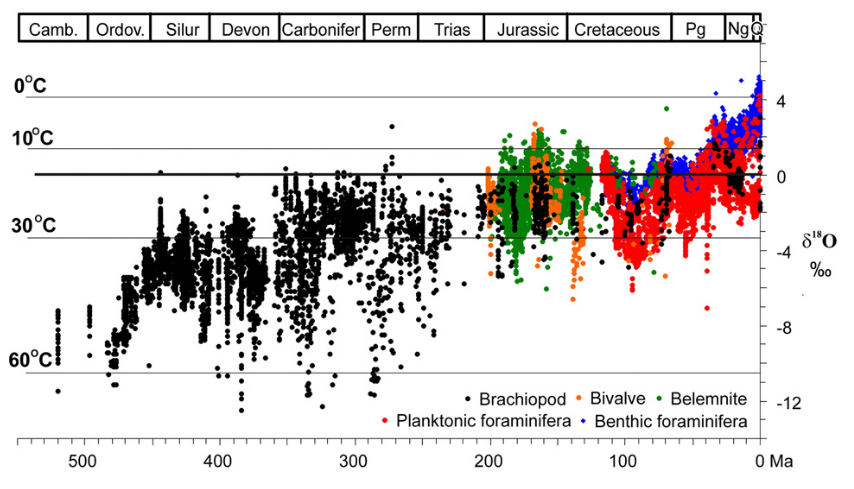
\includegraphics[width=.95\textwidth]{img/veizer2015.png}

\smallskip\noindent\small Zawartość $^{18}$O zmierzona w skamieniałościach i~osadach morskich, wraz z~interpretacją temperaturową przy standardowej kalibracji (lewa oś). Źródło: Veizer et al.~2015.
\end{figure}


Gdyby ten trend interpretować dosłownie, oznaczałby on, że na początku fanerozoiku temperatury (geolodzy z KNG PAN nie piszą, jakiego parametru dotyczy rekonstrukcja, ale można przyjąć że podobnie jak w oryginalnych publikacjach Veizera chodzi o temperaturę powierzchni oceanów na niskich szerokościach geograficznych) bywały wyższe nie o 14, ale o 50 stopni Celsjusza\footnote{Veizer J., Prokoph A.~(2015):~,,Temperatures and oxygen isotopic composition of Phanerozoic oceans'', \doi{10.1016/j.earscirev.2015.03.008}.}. Na wykresie użytym w stanowisku KNG PAN tego trendu nie widać, bo krzywa temperaturowa przedstawia tylko składniki resztowe, a trend liniowy został usunięty. 
	
Paradoks ,,gorącego archaiku'' (który zahacza również o fanerozoik) odkryto pięćdzisiąt lat temu, i do dzisiaj nie udało się rozstrzygnąć, w jaki sposób należy interpretować te dane. Nie będę streszczał całej historii prób rozwiązania tego problemu, ale wspomnę tylko, że są trzy główne hipotezy (czy też grupy hipotez) tłumaczące taki stan rzeczy:
\begin{itemize}
	\item  oceany faktycznie były wtedy takie gorące
	\item zawartość izotopowa $^{18}$O wody morskiej była w odległej przeszłości inna niż obecnie
	\item zawartość izotopowa $^{18}$O skamieniałości/skał osadowych zmieniła się od czasu ich depozycji
\end{itemize}
	
Omówienie tych hipotez zainteresowany czytelnik może znaleźć tutaj\footnote{Tartèse R., et al.~(2017):~,,Warm Archean oceans reconstructed from oxygen isotope composition of early-life remnants'', \doi{https://doi.org/10.7185/geochemlet.1706}.}\footnote{Ryb U., Eiler J.~M.~(2018):~,,Oxygen isotope composition of the Phanerozoic ocean and a possible solution to the dolomite problem'', \doi{10.1073/pnas.1719681115}.}\footnote{Sengupta S., Pack A.~(2018):~,,Three Billion Year Secular Evolution of the Triple Oxygen Isotope Composition of Marine Chert'', \doi{10.1016/j.chemgeo.2018.07.012}.}\footnote{Galili N., et al.~(2019):~,,The geologic history of seawater oxygen isotopes from marine iron oxides'', \doi{10.1126/science.aaw9247}.}.

\begin{figure}
	\centering
	
	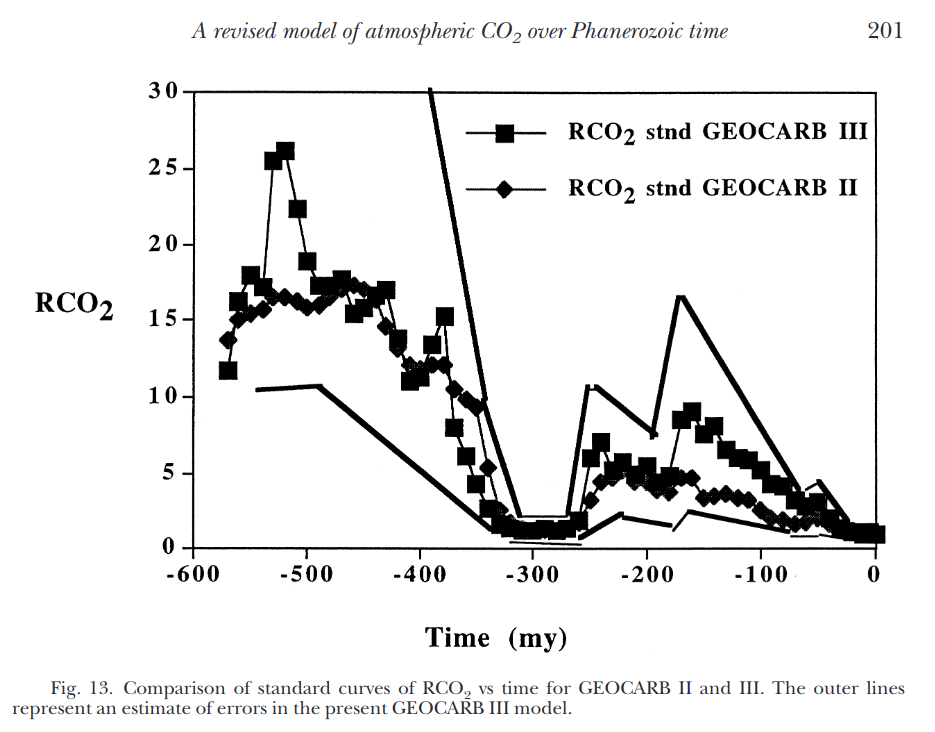
\includegraphics[width=.95\textwidth]{img/berner2001.png}	
	\smallskip\noindent\small Rekonstrukcja poziomu dwutlenku węgla w atmosferze według modelowania GEOCARB III. Linie górna i dolna pokazują zakres niepewności. Skala przedstawia wielokrotność ,,współczesnych'' wartości (ok. 300 ppm). Źródło: Berner i Kovathala, 2001.
\end{figure}

Z kolei rekonstrukcja stężeń CO$_2$ oparta jest o wyliczenia modelu cykli geochemicznych o długim kroku czasowym, i nie ma wystarczającej rozdzielczości by wychwycić zmiany zawartości dwutlenku węgla, które mogły przyczynić się do zlodowacenie w ordowiku\footnote{Shen J., et al.~(2018):~,,Improved efficiency of the biological pump as a trigger for the Late Ordovician glaciation'', \doi{10.1038/s41561-018-0141-5}.}\footnote{Pancost R., et al.~(2013):~,,Reconstructing Late Ordovician carbon cycle variations'', \doi{10.1016/j.gca.2012.11.033}.}\footnote{Pohl, A., et al.~(2016):~,,Glacial onset predated Late Ordovician climate cooling'', \doi{10.1002/2016PA002928}.}; tym bardziej, jeśli była to tak naprawdę seria wymuszanych orbitalnie glacjałów i interglacjałów, analogiczna do tych które mieliśmy w plejstocenie\footnote{Ghienne J-F., et al.~(2014):~,,A Cenozoic-style scenario for the end--Ordovician glaciation'', \doi{10.1038/ncomms5485}}.
	
Geolodzy z KNG PAN powinni też zdawać sobie sprawę z tego, że w odległej przeszłości Słońce świeciło nieco słabiej ($\approx$96{,}5\% obecnej jasności), a inna konfiguracja kontynentów mogła faworyzować inicjowanie zlodowaceń nawet przy relatywnie wysokich, w stosunku do stanu obecnego, poziomach dwutlenku węgla\footnote{Pohl A., et al.~(2014):~,,Effect of the Ordovician paleogeography on the (in)stability of the climate'', \doi{10.5194/cp-10-2053-2014}.}.
		
W opublikowanym cztery lata temu artykule przeglądowym trzech amerykańskich geologów tak opisuje problem ordowiku i ewolucję wiedzy na temat jego przyczyn\footnote{Algeo T.~J., Marenco P., Saltzman M.~R.~(2016):~,,Co-evolution of oceans, climate, and the biosphere during the <<Ordovician Revolution>>: A review'', \doi{https://doi.org/10.1016/j.palaeo.2016.05.015}.}:
		
\begin{quotation}
The Hirnantian glaciation is widely thought to have developed under conditions of high atmospheric pCO$_2$, an idea based largely on the Phanerozoic carbon cycle models of the late Robert Berner (Berner, 1991, 1994, 2006; Berner and Kothavala, 2001) and possibly reinforced by C--isotope studies of soil minerals as CO$_2$ paleobarometers (Yapp and Poths, 1992; Mora et al., 1996). However, this would be highly unusual given the strong positive correlation between low pCO$_2$ and glaciation for the Phanerozoic as a whole (Royer, 2006) and for the Pleistocene in particular (Cuffey and Vimeux, 2001; Shakun et al., 2012). Various hypotheses have been proposed to account for this supposed anomaly, including a weak early Sun (Ramstein, 2011), high cloud albedo caused by cosmic ray flux (Shaviv and Veizer, 2003), and diminished silicate weathering owing to extensive ice cover (Kump et al., 1999). However, it is also possible that the inference of high atmospheric pCO$_2$ during the Hirnantian is simply incorrect: Berner's pCO$_2$ curves have only a 10--Myr resolution and, thus, are likely to have completely missed a short-lived ($\approx$1--Myr--long) pCO$_2$ minimum during the Hirnantian glaciation. The significance of the Yapp and Poths (1992) study is uncertain as well: they studied the late Richmondian (late Katian) Neda Formation, which predated the Hirnantian glaciation by several million years. A recent investigation inferred that pCO$_2$ in the early Katian, ~8 million years prior to the Hirnantian glaciation, was $<8\times$ present atmospheric level (PAL), or less than half of earlier estimates (Pancost et al., 2013). Thus, atmospheric pCO$_2$ during the Hirnantian glaciation may well have been lower than previously thought.	
\end{quotation}

		
W Komitecie Nauk Geologicznych PAN co najmniej kilka osób zna tę przeglądówkę; na przykład prof. Leszek Marynowski z Uniwersytetu Śląskiego jest współautorem cytującego go artykułu, który został opublikowany zaledwie kilkanaście miesięcy temu\footnote{Smolarek--Łach J., et al.~(2019):~,,Mercury Spikes Indicate a Volcanic Trigger for the Late Ordovician Mass Extinction Event: An Example from a Deep Shelf of the Peri-Baltic Region'', \doi{10.1038/s41598-019-39333-9}.}. Nie będę spekulować, co powstrzymało go przed podzieleniem się z kolegami tą wiedzą.

Równie zaskakujące jest to, że wnioski odnośnie przyczyn zmian klimatu w permie autorzy stanowiska KNG PAN wyciągają \emph{wyłącznie} w oparciu o znaleziony w internecie wykres, i najwyraźniej nie skonfontowali go z żadnymi naukowymi publikacjami na ten temat. Przykładowo, wystarczy zajrzeć do numeru specjalnego ,,Palaeogeography, Palaeoclimatology, Palaeoecology'' z ubiegłego roku, poświęconego epoce lodowej późnego palezoiku, by niemal w każdym artykule znaleźć słowa o związku pomiędzy poziomem dwutlenku węgla a deglacjacją na początku permu\footnote{Pod redakcją Qie, W., et al.~(2019): ,,Global events of the Late Devonian to Early Permian'', w \href{https://www.sciencedirect.com/journal/palaeogeography-palaeoclimatology-palaeoecology/vol/531/part/PA}{Palaeogeography, Palaeoclimatology, Palaeoecology}.}. Nieco starszy artykuł przeglądowy Montañez i~Paulsona\footnote{Montañez I.~P., Poulsen C.~J.~(2013):~,,The Late Paleozoic Ice Age:An Evolving Paradigm'', \doi{10.1146/annurev.earth.031208.100118}.} tak podsumowuje opinie geologów na temat przyczyn zmian klimatu w tym okresie:

\begin{quotation}
	The view of the late Paleozoic has evolved from one of long--term stability to one of dynamic change that archives the climate and ecosystem response to repeated glacial-interglacial conditions that were likely CO$_2$ forced. As the most recent transition froman icehouse to a greenhouse world, the late Paleozoic provides a unique analog for ourwarming world.
	
	Both the stepped nature of glaciation during the onset and demise of the LPIA\footnote{\emph{Late Paleozoic Ice Age}, zlodowacenie późnego paleozoiku.} and the temporal distribution of ice centers suggest threshold behavior, likely involving changes in atmospheric pCO$_2$ and orbital forcing analogous to that which occurred during the initiation of the Cenozoic icehouse. Climate model simulations indicate that CO$_2$ was the fundamental driver for the buildup and breakdown of glaciers. Other factors, including topography, may have been locally important.
\end{quotation}

Nie jest to zresztą pomysł nowy, już w klasycznym artykule z~2007 roku Montañez i~jej współautorzy pisali\footnote{Montañez I.~P., et al.~(2007):~,,CO$_2$--Forced Climate and Vegetation Instability During Late Paleozoic Deglaciation'', \doi{10.1126/science.1134207}.Patrz też: Goddéris Y., et al.~(2017): ,,Onset and ending of the late Palaeozoic ice agetriggered by tectonically paced rock weathering'', \doi{10.1038/ngeo2931}.}:

\begin{quotation}
	The late Paleozoic deglaciation is the vegetated Earth’s only recorded icehouse-to-greenhouse transition, yet the climate dynamics remain enigmatic. By using the stable isotopic compositions of soil-formed minerals, fossil-plant matter, and shallow-water brachiopods, we estimated atmospheric partial pressure of carbon dioxide (pCO$_2$) and tropical marine surface temperatures during this climate transition. Comparison to southern Gondwanan glacial records documents covariance between inferred shifts in pCO$_2$,temperature, and ice volume consistent with greenhouse gas forcing of climate. Major restructuring of paleotropical flora in western Euramerica occurred in step with climate and pCO$_2$ shifts, illustrating the biotic impact associated with past CO$_2$--forced turnover to a permanent ice--free world.
\end{quotation}

Nie ma więc wątpliwości, że w środowisku geologów specjalizujących się w badaniu przyczyn zmian klimatu w odległej przeszłości rola dwutlenku węgla nie jest kwestionowana, a opinia geologów z KNG PAN pozostaje, no cóż, ich opinią powstałą przy kawie i ciasteczkach.
	
Zakończę wykresem i cytatem z jeszcze jednego artykułu z ubiegłego roku\footnote{Mills, B.~J., et al.~(2019):~,,Modelling the long-term carbon cycle, atmospheric CO$_2$, and Earth surface temperature from late Neoproterozoic to present day'', \doi{10.1016/j.gr.2018.12.001}.}, który zawiera dokładnie takie porównanie zmian klimatu oraz poziomu CO$_2$, jakie \emph{powinno} znaleźć się w stanowisku Komitetu Nauk Geologicznych: uwzględniające niepewności, różne rekonstrukcje oparte zarówno o modelowanie geochemiczne, jak i proxy paleoklimatyczne, i badający czułość konkluzji od przyjętych założeń.

\begin{figure}
	\centering
	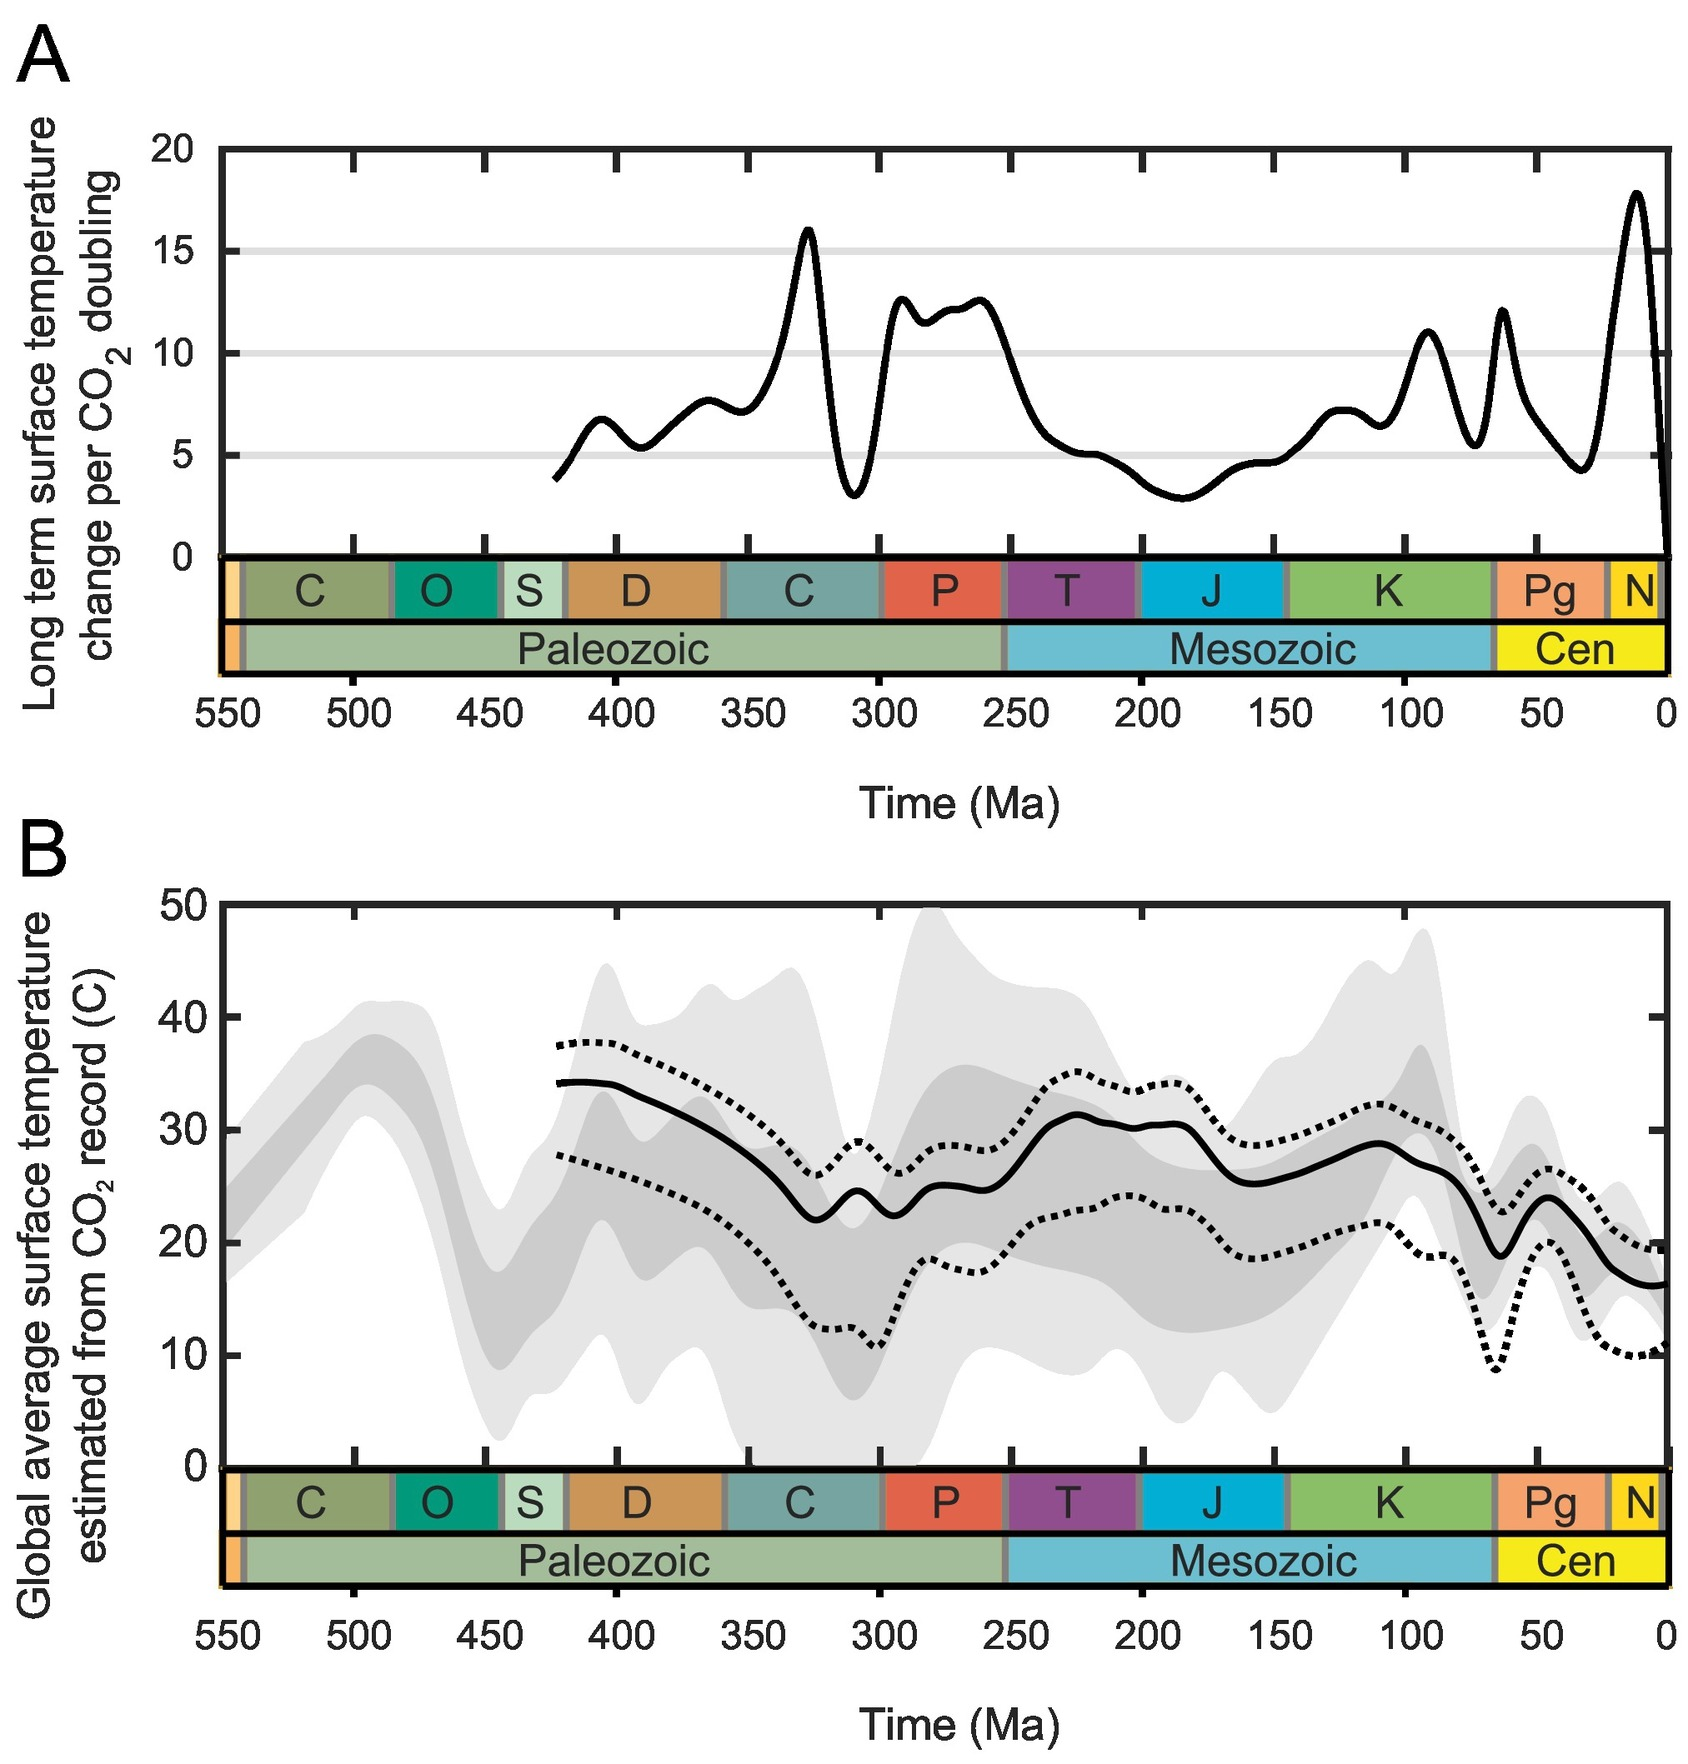
\includegraphics[width=.95\textwidth]{img/phan2019.png}	
	
	\smallskip\noindent\small Panel górny: zależność dwutlenku węgla od średniej temperatury globalnej, zdiagnozowana w oparciu o dane proxy. Panel dolny: rekonstruowana średnia temperatura Ziemi (zakres koloru szarego) oraz temperatura wyliczona w oparciu o równowagową czułość klimatu (ESS) 5K/podwojenie CO$_2$ (kolor czarny). Źródło: Mills et al. (2019).
\end{figure}

Jak piszą jego autorzy:

\begin{quotation}
	By compiling independent proxy records of global average surface temperature and atmospheric CO$_2$ concentration for the Phanerozoic, we have shown that when accounting for the solar flux, long--term Phanerozoic surface temperature changes can be clearly related to variations in the CO$_2$ greenhouse (Fig.~6). CO$_2$ appears to be a primary driver of climate on geological timescales (e.g.~Royer et al., 2004).
\end{quotation}		

\newpage

\subsection*{Zmiany klimatu ciągu ostatnich 800 tysięcy lat}

Wiedza autorów stanowiska Komitetu Nauk Geologicznych na temat zmian klimatu plejstocenu również pozostawia wiele do życzenia.

\begin{quotation}
	\textbf{Zmienność temperatur w skali setek tysięcy lat (plejstocen)}

	Dla ostatnich 800 tys.~lat są dostępne informacje o poziomie CO$_2$ i~temperaturze oparte o analizę powietrza uwięzionego w lodzie Antarktydy (projekty EPICA i~Vostok). Wartość paleotemperatur określono  metodą stosunków izotopów tlenu $^{16}$O/$^{18}$O. Obie wartości (CO$_2$ oraz T\si{\celsius}) są  silnie skorelowane, ale wzrost temperatury z reguły nieznacznie wyprzedza wzrost poziomu CO$_2$ (Fig.~2). Od ok.~450 tys.~lat miały miejsce cztery pełne cykle ocieplenia klimatu do podobnego (a nawet wyższego) poziomu temperatury, jaki jest obserwowany obecnie, i~wzrostu stężenia CO$_2$ do wartości ok.~300 ppm. Piąta analogiczna faza zaczęła się ok.~12 tys.~lat temu i~znajduje się na etapie maksimum temperaturowego. Amplituda zmian temperatury w plejstocenie sięgała 10\si{\celsius} i z pewnością nie była spowodowana działalnością człowieka. Uważa się, że przyczyną były okresowe zmiany parametrów orbitalnych Ziemi w~jej obiegu wokół Słońca (tzw.~cykle Milankowicza). Te obserwacje zdają się wskazywać, że wzrost poziomu CO$_2$ w~atmosferze do wartości ok.~300 ppm jest raczej skutkiem niż przyczyną wzrostu temperatury globu, co nie wyklucza sprzężenia zwrotnego: wzmacniania trendu wzrostowego temperatury przez CO$_2$.
\end{quotation}

Niby tak, ale nie do końca, bo niemal każde zdanie zawiera jakąś nieścisłość.

Po pierwsze brakuje informacji, że na wykresie przedstawiono \emph{lokalne} zmiany temperatury, rekonstruowane dla lokalizacji z której dokonano odwiertu, i lokalnych wartości dotyczy odnotowana amplituda 10\si{\celsius}. Zmiany globalne miały amplitudę mniejszą, najnowsze oszacowania\footnote{Tierney J., et al.~(2020):~,,Glacial cooling and climate sensitivity revisited'', \href{preprint}{https://eartharxiv.org/me5uj/}. To jeszcze nierecenzowany preprint, ale zawiera też syntezę innych świeżych prac na ten temat.} wskazują że było to około 6\si{\celsius}. 

Po drugie, rekonstrukcja temperatury jest oparta o analizę zawartości ciężkiego izotopu wodoru (deuteru), a nie tlenu $^{18}$O w cząsteczkach wody tworzących lądolód\footnote{Jouzel J., et al.~(2007):~,,Orbital and Millennial Antarctic Climate Variability over the Past 800,000 Years'', \doi{10.1126/science.1141038}.}. Gdyby geolodzy z KNG PAN sięgnęli do artykułu opisującego te dane, zamiast opierać się o znaleziony w internecie pierwszy lepszy obrazek, zapewne nie popełniliby takiej pomyłki.

Po trzecie, choć rekonstruowane zmiany temperatury na Antarktydzie poprzedzały wzrost zawartości dwutlenku węgla w atmosferze, nie jest to prawdą w odniesieniu do średniej temperatury \emph{całego} globu\footnote{Shakun J.~D., et al.~(2012):~,,Global warming preceded by increasing carbon dioxide concentrations during the last deglaciation'', \doi{10.1038/nature10915}.}.

Po czwarte, poziom 300 ppm został w ciągu ostatnich 800 tysięcy lat osiągnięty tylko dwukrotnie: 335 tysięcy lat temu, oraz 108 lat temu\footnote{Bereiter B., et al.~(2015):~,,Revision of the EPICA Dome C CO$_2$ record from 800 to 600 kyr before present'', \doi{10.1002/2014GL061957}, L\"{u}thi D., et al.~(2008):~,,High-resolution carbon dioxide concentration record 650,000--800,000 years before present'', \doi{10.1038/nature06949}.}. O ile w pierwszym przypadku przyczyny tego były naturalne, to wzrost zawartości dwutlenku węgla mierzony od początku ery industrialnej naturalny oczywiście nie jest. Więcej na ten temat w~dalszej części komentarza.

\newpage

\subsection*{Zmiany klimatu ciągu ostatnich 2 tysięcy lat}

\begin{quotation}
	\textbf{Zmienność temperatur w skali setek lat (okres historyczny)}

	W ramach piątego maksimum klimatycznego, w którym się znajdujemy, temperatura na Ziemi rośnie od min.~300 lat (Fig.~3), począwszy od minimum klimatycznego tzw. Małej Epoki Lodowej (MEL, ang.~LIA). W okresie MEL, ludzie przemieszczali się zimą saniami poprzez całkowicie zamarznięty Bałtyk. Z kolei przed MEL, ok.~850 lat temu, ludzkość doświadczała  uroku Średniowiecznego Optimum Klimatycznego, kiedy temperatura na Ziemi była wyższa niż obecnie.
\end{quotation}

\begin{figure}
	\centering
	
	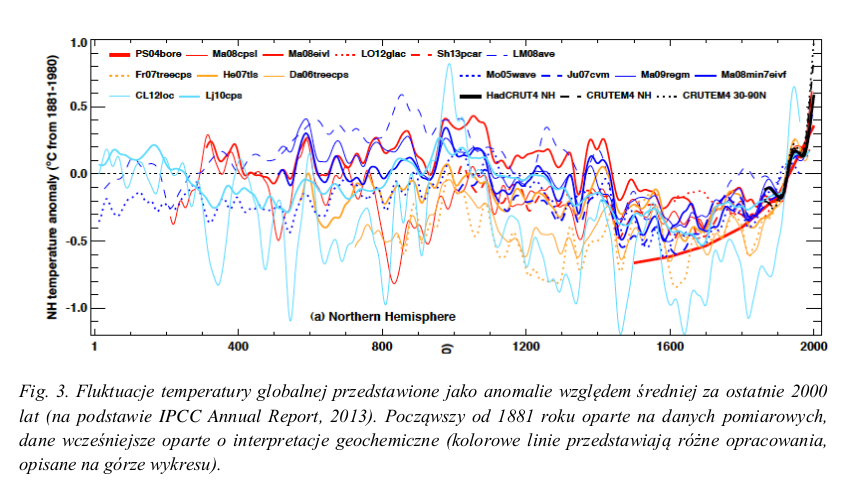
\includegraphics[width=.95\textwidth]{img/kng2.png}	
\end{figure}


Zacznijmy od wykresu. KNG PAN oznaczyło jako jego źródło ,,IPCC Annual Report, 2013'', choć tak naprawdę jest to ,,Climate Change 2013: The Physical Science Basis. Contribution of Working Group I to the Fifth Assessment Report of the Intergovernmental Panel on Climate Change'' (rozdział piąty, rys.~5{.}7), i nie jest raportem rocznym (te zawierają sprawozdania finansowo-organizacyjne panelu). Podpisało go też jako ,,fluktuacje temperatury globalnej'', mimo że nawet na samym wykresie jest przecież etykieta ,,półkula północna''. Ta pomyłka jest tym dziwniejsza, że kompletna ilustracja z raportu IPCC zawiera wykres również dla temperatury globalnej:

\begin{figure}
	\centering
	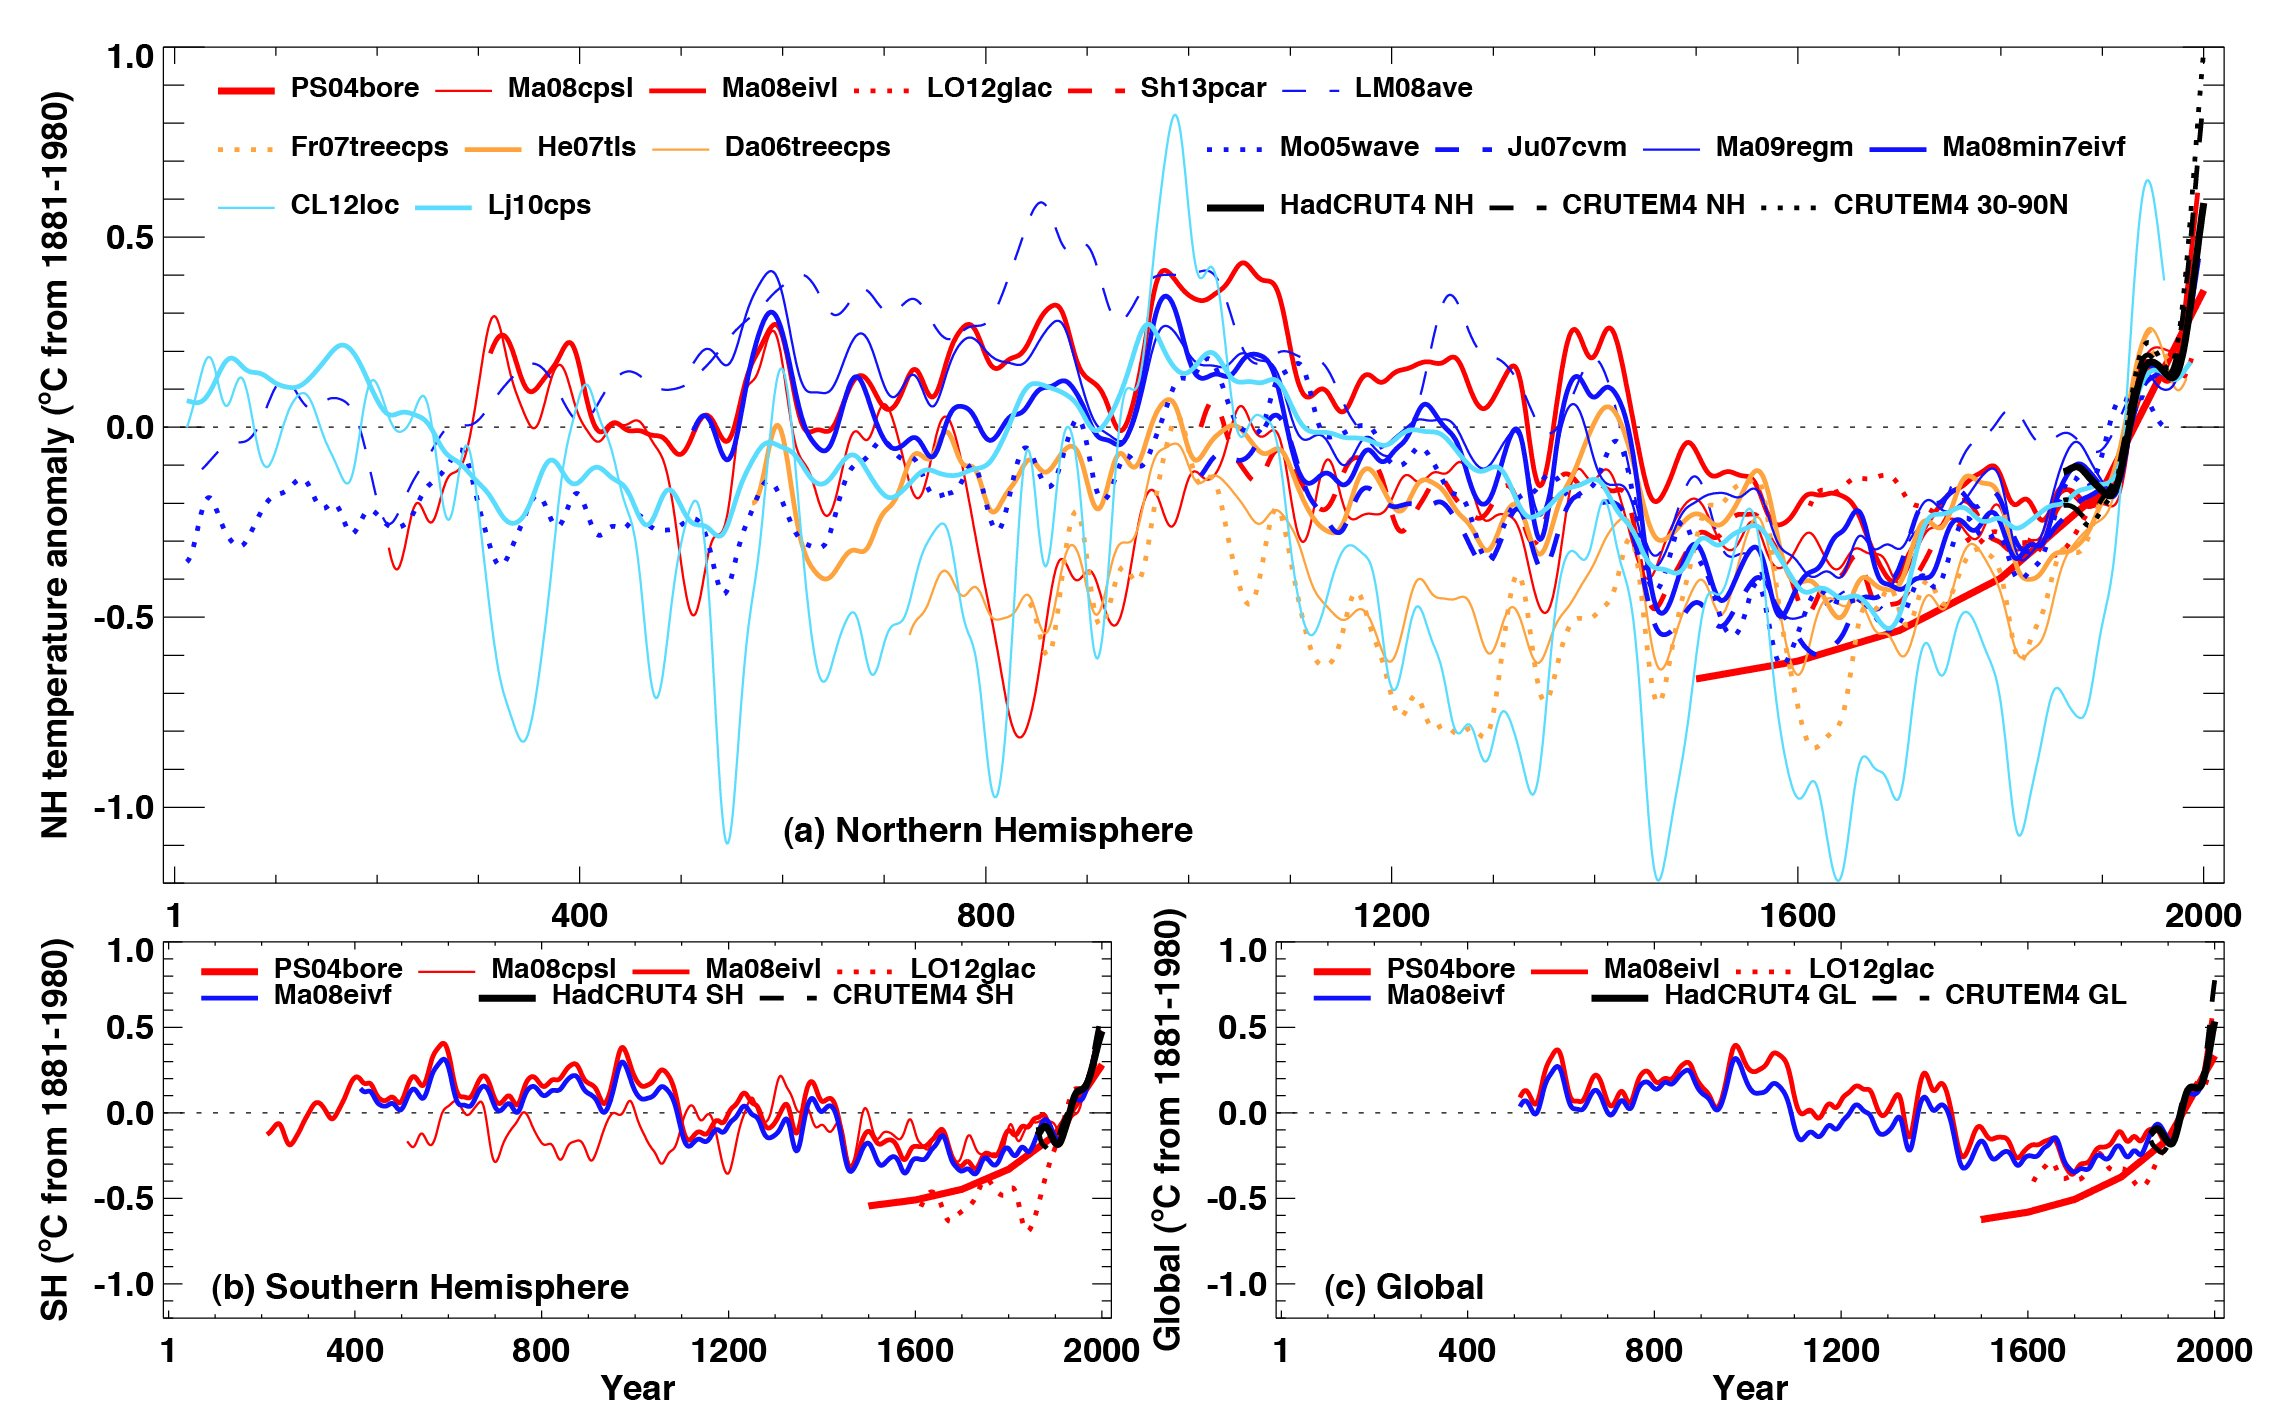
\includegraphics[width=.95\textwidth]{img/Fig5-07.jpg}	
\end{figure}
		
Podejrzewam więc, że autorzy stanowiska KNG PAN nie widzieli tego wykresu w oryginale, tylko skorzystali z okrojonej wersji którą gdzieś znaleźli w internecie. Co gorsza, nie jestem nawet pewien, czy dobrze się mu przyjrzeli, skoro twierdzą że 850 lat temu ,,temperatura na Ziemi była wyższa niż obecnie''. Wykres pokazuje, że była niższa, zarówno na obszarze samej półkuli północnej, jak i całego globu. Naukowców z KNG PAN zmyliło jak sądzę to, że przedstawiono na nim trzy grupy rekonstrukcji: te obejmujące całą półkulą północną, obejmujące tylko powierzchnię lądów, i obejmujące tylko powierzchnię lądów powyżej trzydziestego równoleżnika północnego. Cienka niebieska linia (oznaczona jako ,,CL12loc''), która pokazuje najcieplejsze średniowiecze, to rekonstrukcja z pracy ,,The extra--tropical Northern Hemisphere temperature in the last two millennia: reconstructions of low--frequency variability'' Christiansena i Ljungqvista\footnote{Christiansen B.~i~Ljungqvist F.~C.~(2012):~,,The extra-tropical Northern Hemisphere temperature in the lasttwo millennia: reconstructions of low-frequency variability'', \doi{10.5194/cp-8-765-2012}.}, która była oparta wyłącznie o~proxy lądowe spoza tropików półkuli północnej, i~powinna być porównywana z obserwacjami przeprowadzonymi na tym samym obszarze (czarna linia kropkowana). Amplituda zmian temperatury na wyższych szerokościach geograficznych była większa, ale wyższe jest też obecne tempo ocieplenia lądów; i~dawno już przewyższyło maksymalny poziom osiągnięty w tej rekonstrukcji.
		
Dziwi mnie też, że geolodzy z KNG PAN nie cytują ustaleń PAGES2k. Można byłoby przecież oczekiwać, że jeśli ktoś chciałby podsumować stan badań nad zmianami klimatu z ostatnich 2000 lat, to powinien wiedzieć o dużym międzynarodowym projekcie poświęconym \emph{dokładnie} temu zagadnieniu, którego najnowsze ustalenia opublikowano w ubiegłym roku. Oczywiście, gdyby geolodzy z KNG PAN zajrzeli do publikacji PAGES2k, odkryliby że współczesne globalne ocieplenie jest nie tylko najcieplejszym okresem naszej ery\footnote{PAGES2k Consortium (2019):~,,Consistent multidecadal variability in global temperature reconstructions and simulations over the Common Era'', \doi{10.1038/s41561-019-0400-0}.}, ale też jedynym, w którym ocieplenie następuje niemal na całej powierzchni planety\footnote{Neukom R., et al.~(2019):~,,No evidence for globally coherent warm and cold periods over the preindustrial Common Era'', \doi{10.1038/s41586-019-1401-2}.}.
		
Zamiast tego wolą opowiadać bajki o podróżach saniami przez całkowicie zamarznięty Bałtyk.

\begin{quotation}
	Zasadniczą różnicą między okresowymi wzrostami temperatury globalnej w ciągu ostatniego miliona lat a czasami współczesnymi wydaje się być tempo tych zmian. Uważa się, że dziś jest ono znacząco wyższe niż dawniej. Niepewność polega na tym, że nie potrafimy porównać dawnej dynamiki wzrostu temperatury i koncentracji CO$_2$ z dynamiką dzisiejszą. Współcześnie mamy do dyspozycji długie i~ciągłe serie czasowe pomiarów temperatury, które wykonujemy termometrami naziemnymi lub przyrządami umieszczanymi na satelitach bądź w balonach o zasięgu stratosferycznym. Informacje o temperaturze na dawnej Ziemi pozyskujemy metodami pośrednimi, których wyniki są obarczone niepewnością co do rzeczywistej wartości temperatury oraz czasu (wieku geologicznego). Jest zatem możliwe, że dawniej tempo zmian temperatury było podobne do dzisiejszego, ale niepełne ciągi danych, założenia metodyczne oraz uśrednienia i uogólnienia interpretacyjne nie pozwalają na pełną obserwację rzeczywistych przebiegów zmian temperatury i koncentracji CO$_2$. W konsekwencji, obserwowane współcześnie tempo wzrostu temperatury nie może być traktowane jako dowód na to, że naturalny proces wzrostu temperatury na Ziemi został w zauważalnym stopniu wzmocniony przez efekt cieplarniany, związany z antropogenicznym CO$_2$. Wskazuje na to również wyraźny epizod ocieplenia w latach trzydziestych dwudziestego wieku — na terytorium dzisiejszej Polski zanotowano wówczas najwyższe temperatury, odnotowane ponownie dopiero w 2019 roku.
\end{quotation}

Wypada zacząć od tego, że obserwowane współcześnie tempo wzrostu temperatury nie jest \emph{samo w sobie} dowodem tego, że ocieplenie jest konsekwencją wzmocnienia efektu cieplarnianego. Dowody potwierdzające dominującą rolę czynników antropogenicznych opierają się o porównanie przewidywań teoretycznych zmian klimatu ze zmianami rzeczywistymi, zarówno w czasie jak i przestrzeni\footnote{Np.~Jones G.~S., Stott P.~A., Christidis N.~(2013):~,,Attribution of observed historical near--surface temperature variations to anthropogenic and natural causes using CMIP5 simulations'', \doi{10.1002/jgrd.50239}.}. Gdyby ludzkość emitowała mniej dwutlenku węgla, i w konsekwencji zawartość tego gazu w atmosferze rosła znacznie wolniej, obserwowalibyśmy ocieplenie przebiegające w wolniejszym tempie (jest nawet hipoteza, zwana ,,wczesnym antropocenem'', która postuluje że coś takiego zdarzyło się w połowie holocenu, dzięki deforestacji, rozwojowi rolnictwa i~hodowli bydła\footnote{Ruddiman W.~F.~(2013):~,,The Anthropocene'', \doi{annurev-earth-050212-123944}.}. Szybkie tempo zmiany klimatu ułatwia natomiast badanie ich przyczyn, bo dzięki zwiększeniu stosunku sygnału do szumu nie musimy prowadzić długich obserwacji, aby statystycznie potwierdzić przewidywany efekt.

Mierzony w ostatnich kilku dekadach trend temperatury globalnej wynosi około 0{,}02\si{\celsius} rocznie, czyli 2 stopnie na stulecie. Możemy spokojnie wykluczyć, że podobne globalne ocieplenie trwające \emph{dłużej} niż 1000 lat zaszło w ciągu ostatnich kiludziesięciu milionów lat: oznaczałoby to zmianę średniej temperatury globalnej o ponad 20 stopni Celsjusza, co spowodowałoby masowe wymieranie wielu gatunków, i byłoby łatwo dostrzegalne w zapisie kopalnym \emph{nawet jeśli} rozdzielczość czasowa rekonstrukcji zmiany temperatury nie pozwalałaby na stwierdzenie, że do wzrostu temperatury doszło.

Z drugiej strony, możemy też z dużym prawdopodobieństwem wykluczyć, aby takie tempo wzrostu temperatur było podtrzymane dłużej niż 50 lat w ciągu ostatnich 2000 lat, co prowadziłoby do zmian o amplitudzie 1\si{\celsius}. Gdyby coś takiego miało miejsce, byłoby to widoczne na przykład w rekonstrukcji PAGES2k, o której mowa powyżej.

Pomiędzy tymi dwoma skrajnymi przypadkami rozciąga się przestrzeń możliwych trendów o długości od kilkudziesięciu do powiedzmy stu czy dwustu lat z gorzej poznanych okresów, które mogłyby być niewykryte w danych proxy, na przykład sprzed kilku czy kilkuset tysięcy lat. W praktyce możemy uznać, że jest to mało prawdopodobne: jak pisałem w poprzedniej części komentarza, każda zmiana klimatu ma swoją przyczynę, i aby spowodować ocieplenie analogiczne w skali do obecnego, takimi przyczynami mógłby być tylko bardzo szybki (w skali geologicznej) wzrost zawartości gazów cieplarnianych w atmosferze, albo bardzo szybki wzrost jasności Słońca, co najmniej o 1\%.

Szybki wzrost poziomu dwutlenku węgla w atmosferze byłby zauważalny w rekonstrukcjach składu atmosfery opartych o rdzenie lodowe (nawet przy zmniejszonej amplitudzie, będącej konsekwencją dyfuzji powietrza w firmie); możemy więc znów z dużą dozą pewności wykluczyć, że taki wzrost zdarzył się w ciągu ostatnich 800 tysiącach lat. Oczywiście, dwutlenek węgla nie mógłby się w atmosferze pojawić znikąd, i nie jest łatwo wymyślić, co mogłoby być źródłem porównywalnym ilościowo z 650 gigatonami węgla, które zostały przez ludzkość uwolnione do atmosfery w ciągu ostatnich 200 lat. Używając proxy geochemicznych można oszacować, że maksymalne tempo emisji dwutlenku węgla do atmosfery w ciągu ostatnich 66 milionów lat było o rząd wielkości mniejsze, niż obecne emisje antropogeniczne\footnote{Zeebe R.~E., Ridgwell A., Zachos J.~C.~(2016):~,,Anthropogenic carbon release rate unprecedented during the past 66 million years'', \doi{10.1038/ngeo2681}.}, a~zatem i~spowodowana przez nie zmiana klimatu miała mniejsze tempo niż obecne ocieplenie.

Analogicznie, istniejące rekonstrukcje aktywności słonecznej dla okresu holocenu ($\approx11$ tysięcy lat) wskazują, że zmienność irradiancji słonecznej w tym okresie jest o rząd wielkości mniejsza od wymaganego 1\%\footnote{Np.~Rooth R., Joos F.~(2013):~,,A reconstruction of radiocarbon production and total solar irradiance from the Holocene $^{14}$C and CO$_2$ records: implications of data and model uncertainties'', \doi{10.5194/cp-9-1879-2013}, Vieira L.~E.~A., et al.~(2011):~,,Evolution of the solar irradiance during the Holocene'', \doi{0004-6361/201015843}.}. Dłuższych serii proxy słonecznych (na razie) nie mamy\footnote{Rekonstrukcje aktywności słonecznej opierają się o relacje statystyczne pomiędzy liczbą plam słonecznych, oraz tempem produkcji radioaktywnych izotopów $^{14}$C i $^{10}$Be w atmosferze przez cząstki promieniowania kosmicznego, które modulowane jest intensywnością pola magnetycznego Słońca, i które można oszacować badając zawartość tych izotopów w słojach drzew i rdzeniach lodowych. Systematyczne liczenie plam słonecznych zaczęło się niespełna 400 lat temu; a izotopy $^{14}$C i $^{10}$Be mają ograniczoną użyteczność przed początkiem holocenu. Pewne nadzieje wiąże się z proxy opartym o zawartość jonów azotanowych z rdzeni lodowych, ale na razie nie opracowano jeszcze wykorzystujących ich rekonstrukcji.}, więc można sobie wyobrazi scenariusz, w którym kilka milionów lat temu doszło, na tylko 100 czy 200 lat, do nagłego pojaśnienia Słońca, co doprowadziło do krótkotrwałego globalnego ocieplenia o skali i tempie porównywalnym z obecnym, po czym jasność równie szybko spadła, powodując spadek temperatury zanim doszło do zmian środowiska, które zostawiłyby ślad w zapisie geologicznym (jak np. stopnienie części lądolodów i zmiana oceanicznego $\delta^{18}$O). Podkreślę jednak, że nie ma jednak żadnych dowodów na to, że coś takiego się zdarzyło, więc jest to scenariusz czysto spekulatywny.

Nawet jednak gdyby coś takiego się faktycznie dawno temu zdarzyło, to nie ma to żadnego związku z przyczynami \emph{obecnej} zmiany klimatu. Wiemy przecież, jak zmieniała się aktywność słoneczna w ostatnich dekadach, i że nie może być ona odpowiedzialna za obserwowane ocieplenie. Wiemy też, że ludzkość spowodowała wzrost zawartości dwutlenku węgla i innych gazów cieplarnianych w atmosferze, i~że wynikający z tego wzrost temperatury w zupełności wystarcza, by wytłumaczyć obserwowane zmiany.

Fragmentu o ociepleniu w Polsce w latach 30-tych dwudziestego wieku nie rozumiem, i nie wiem co ma wspólnego z resztą wywodu geologów KNG PAN. Miniona dekada 2010--2019 była średnio o 1{,}2\si{\celsius} cieplejsza od lat 30--tych (zarówno jeśli chodzi o temperatury roczne, jak i letnie), chociaż faktycznie lata 30--te były \emph{wówczas} najcieplejszym okresem od początku prowadzenia obserwacji. Lokalne zmiany temperatur charakteryzują się jednak znacznie większą wariancją niż średnie obliczane dla obszaru całej planety, i~nie powinno nikogo dziwić, że na długoletni trend nałożona jest krótkookresowa zmienność wystarczająca, by raz na na jakiś czas wygenerować rekord temperatury maksymalnej.

\newpage

\subsection*{Zmiany klimatu ciągu ostatnich 200 lat}

\begin{quotation}
	Od ok.~1958 roku poziom CO$_2$ w atmosferze (316 ppm, punkt początkowy tzw. krzywej Keelinga, bliski średniej z poprzednich okresów maksymalnego ocieplenia: Fig. 2) zaczął rosnąć i w roku 2018 osiągnął poziom 413 ppm. Wzrost ten jest silnie skorelowany z antropogeniczną emisją CO$_2$ oraz ze wzrostem temperatury. Wzrost temperatury zaczął się jednak ok. 1920, czyli 30 lat wcześniej, a jego poziom, póki co, nie odbiega znacząco od poziomów znanych z poprzednich cykli ocieplenia. Średnia temperatura mierzona w dolnych warstwach atmosfery oscyluje w ciągu ostatnich 40 lat wokół średniej wieloletniej (Fig.~4), choć z drugiej strony, ostatnie dwie dekady były cieplejsze niż wyliczona średnia wieloletnia. Naszym zdaniem dane te przekonywująco dowodzą, że wzrost poziomu CO$_2$ w atmosferze wiąże się z działalnością człowieka, natomiast nie stanowią twardego dowodu, że wzrost temperatury jest jedynie wynikiem wzrostu poziomu CO$_2$. IPCC (cyt. za Annual Report 5) wyciągnął z tych danych odmienny wniosek: ,,The best estimate of the human induced contribution is similar to the observed warming over this period''. Według IPCC można zatem wykazać, że ten wzrost jest spowodowany działalnością człowieka, aczkolwiek sami autorzy Raportu stwierdzają, że związek pomiędzy działalnością człowieka a wzrostem temperatury jest tylko ,,prawdopodobny'' (\emph{Anthropogenic forcings have likely made a substantial contribution to surface temperature increases since the mid--20th century over every continental region except Antarctica}).
\end{quotation}

Stanowisko KNG PAN sugeruje tutaj, że do końca lat 50--tych XX wieku poziom dwutlenku węgla w atmosferze był bliski maksimum z poprzednich interglacjałów, i zaczął rosnąć dopiero w 1958 roku. Nie jest to interpretacja właściwa: kiedy Charles Keeling zaczął prowadzić systematyczne pomiary na Mauna Loa, koncentracja CO$_2$ była już daleko poza zakresem naturalnych wahań w końcu plejstocenu.

\begin{figure}
	\centering
	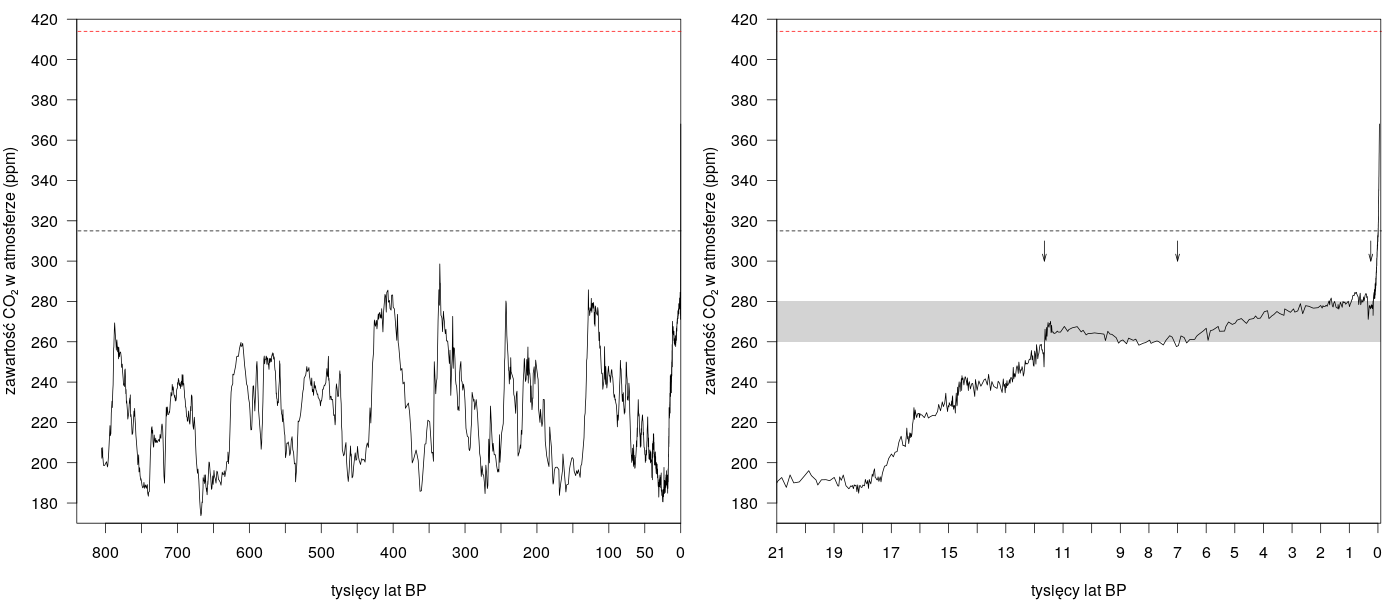
\includegraphics[width=.95\textwidth]{img/icecoreco2ab.png}
	
	\smallskip\noindent\small Zmiany zawartości dwutlenku węgla w atmosferze w oparciu o kompilację kilku rdzeni lodowych z Antarktydy. Wykres lewy pokazuje 800 tysięcy lat, wykres prawy zbliżenie na koniec ostatniej epoki lodowej i holocen. Linia przerywana czarna oznacza poziom z 1958 roku, linia przerywana czerwona poziom z roku 2020.
\end{figure}

W samym holocenie poziom dwutlenku węgla najpierw osiągnął 270 ppm, w ciągu 3 tysięcy lat spadł o 10 ppm, po czym znowu zaczął rosnąć około 7 tysięcy lat temu, osiągając 280 ppm na początku naszej ery. Wraz ze wzrostem liczby ludności oraz nastaniem ery industrialnej szybko rosnąca emisja dwutlenku węgla, zarówno ze spalania paliw kopalnych, jak i wylesiania, spowodowała opuszczenie zakresu naturalnej zmienności wahań CO$_2$ już po roku 1800. W momencie rozpoczęcia pomiarów przez Keelinga, 150 lat później, był już o 35 ppm wyższy niż wartości przedindustrialne.

\begin{figure}
	\centering
	
	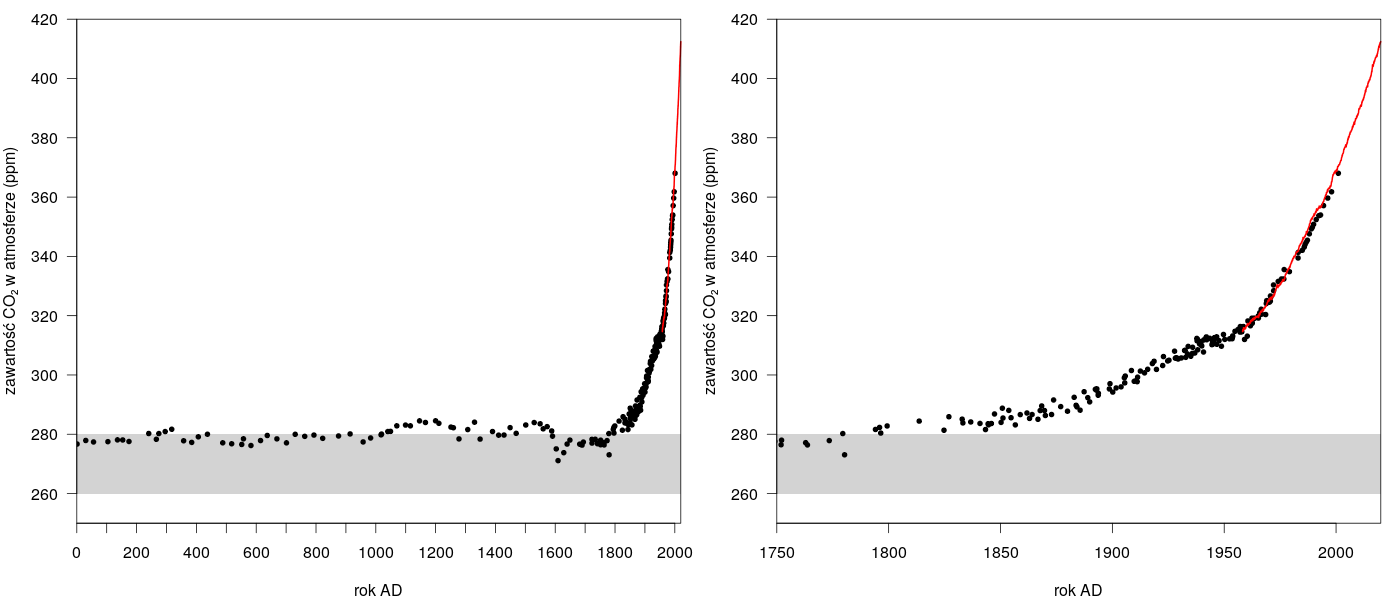
\includegraphics[width=.95\textwidth]{img/icecoreco2cd.png}	
	
	\smallskip\noindent\small Jak wyżej, ale pokazano ostatnie 2020 i 270 lat. Średnie roczne wartości zmierzone na Mauna Loa narysowano kolorem czerwonym.
\end{figure}
		
Nie powinno więc dziwić, że wzrost temperatury planety nie zaczął się w latach 50-tych, tylko znacznie wcześniej. Wymuszenie radiacyjne związane ze wzrostem poziomu dwutlenku węgla z 280 do 300 ppm (czyli stanu z początku XX w.) można oszacować na około 0{,}37 W/m$^2$\footnote{Etminan M., et al.~(2016):~,,Radiative forcing of carbon dioxide, methane, and nitrous oxide: A significant revision of the methane radiative forcing'', \doi{10.1002/2016GL071930}.}, co przy założeniu standardowego zakresu czułości klimatu (1{,}5--4{,}5\si{\celsius} na podwojenie CO$_2$) odpowiadałoby równowagowej zmianie temperatury globalnej o 0{,}28$\pm$0{,}18 stopnia Celsjusza. W połączeniu z naturalną zmiennością klimatu, oraz wymuszeniami radiacyjnymi naturalnego pochodzenia, wystarcza to w zupełności do wytłumaczenia wzrostu temperatury, który nastąpił w pierwszej połowie XX wieku i wcześniej. Bardziej skomplikowane obliczenia, prowadzące do podobnych wniosków, można znaleźć np.~w artykułach Abrama i in.\footnote{Abram N.~J., et al.~(2016):~,,Early onset of industrial--era warming across the oceans and continents'', \doi{10.1038/nature19082}.}, oraz Hausteina i in.\footnote{Haustein K., et al.~(2019):~,,A Limited Role for Unforced Internal Variability in Twentieth-Century Warming'', \doi{10.1175/JCLI-D-18-0555.1}.}.
		
Wbrew temu co twierdzą geolodzy z KNG, średnia temperatura dolnej troposfery w ostatnich 40 latach nie oscylowała wokół średniej wieloletniej (z niezrozumiałych dla mnie powodów stanowisko znów zawiera wykres z bloga, który w dodatku kończy się w lutym 2018). W zależności od użytej serii pomiarowej, trend liniowy temperatury globalnej w okresie 1979--2019 wynosił od 0{,}13 do 0{,}21 stopnia na dekadę\footnote{Seria TLT UAH v6{.}0 \url{https://www.nsstc.uah.edu/data/msu/v6.0/tlt/}.}\footnote{Seria TLT RSS v4{.}0 \url{http://images.remss.com/msu/msu\_time\_series.html}.}.
		
Zwrócę jeszcze uwagę, że autorzy stanowiska KNG nie zrozumieli wniosków zawartych w raporcie IPCC (przy okazji, ,,AR'' to skrót od ,,Assessment Report'', a nie ,,Annual Report''). ,,Bardzo prawdopodobny'' z pierwszego cytatu odnosi się do \emph{globalnego} wzrostu temperatury, ,,prawdopodobny'' zaś do trendów regionalnych, gdzie prób atrybucji dokonywano dla każdego kontynentu osobno\footnote{IPCC (2013):~,,Climate Change 2013: The Physical Science Basis. Contribution of Working Group I to the Fifth Assessment Report of the Intergovernmental Panel on Climate Change'', sekcja ,,10.3.1.1.4 Attribution of regional surface temperature change'' w rozdziale dziesiątym (\href{https://www.ipcc.ch/site/assets/uploads/2018/02/WG1AR5\_Chapter10\_FINAL.pdf}{link}).}. Ponieważ wariancja szeregów czasowych temperatury wzrasta w mniejszych skalach przestrzennych, udowodnienie że \emph{lokalne} ocieplenie zostało spowodowane przez człowieka jest trudniejsze, a zatem i~poziomy ufności są inne.

\newpage

\subsection*{O debacie klimatycznej}

\begin{quotation}
Temperaturą na powierzchni Ziemi rządzi Słońce. Nasłonecznienie (insolacja) jest zależne od aktywności naszej gwiazdy. Im większa aktywność, tym więcej emitowanej energii i tym wyższa temperatura na Ziemi. Aktywność Słońca maleje od kilku (jedenastoletnich) cykli słonecznych, jednak mimo to temperatura na Ziemi nie spada. To zjawisko może niepokoić. Zgodnie bowiem z trendem aktualnego cyklu Milankowicza, wzmocnionego malejącą insolacją, temperatura na Ziemi powinna spadać i powinniśmy zmierzać w kierunku kolejnego glacjału (Fig.~5, linia fioletowa). Jest jednak odwrotnie, czego dowodzą dane obserwacyjne ostatnich dekad, nie tylko fizyczne, ale i przyrodnicze. Takie przyrodnicze przesłanki pozwalają sformułować hipotezę, że wzrost temperatury w ciągu ostatnich dekad jest powiązany przyczynowo z działalnością człowieka. Mimo to, trwa jednak naukowa dyskusja, w jakim stopniu CO$_2$ jest odpowiedzialny za wzrost temperatury (Curry \& Webster, 2011). Na przykład, Monnin et al.~(2004) wskazują na stopniowy spadek temperatury na Ziemi od ok.~5000 lat, przy jednoczesnym wzroście koncentracji CO$_2$ i CH$_4$ (Fig.~5). Z kolei współczesny wzrost temperatury i gazów cieplarnianych bardzo przypomina sytuacje z okresu preborealnego, kiedy pomiędzy 11 500 a 11 000 lat poziom koncentracji CO$_2$ oraz temperatura dynamicznie rosły, aczkolwiek bez ingerencji człowieka (Fig.~5).
\end{quotation}

Jest prawdą, że Słońce jest głównym źródłem energii napędzającej ziemski system klimatyczny. Aby jednak wytłumaczyć \emph{zmiany} temperatury aktywnością słoneczną, aktywność ta też musiałaby być zmienna, a jak wyjaśniałem we wcześniejszym komentarzu, mierzony zakres zmian irradiancji (a także rekonstruowane wartości dla wieków ubiegłych) jest niewystarczający, by spowodować duże zmiany temperatury. Tym bardziej, że aktywność słoneczna, jak sami zauważają geolodzy z KNG, w ostatnich dekadach spada.

Co do ,,naukowej dyskusji'' o roli dwutlenku węgla, KNG PAN znowu wprowadza w błąd opinię publiczną. Niemal wszyscy aktywni zawodowo klimatolodzy akceptują, że to czynniki antropogeniczne odpowiadają za obserwowany w ostatnim stuleciu długoterminowy wzrost temperatur; ,,niemal wszyscy'', bo istnienie konsensusu naukowego w dowolnej dziedzinie nie wyklucza istnienia jednostek, które taki stan rzeczy kontestują. Przykładowo, choć zdecydowana większość geologów akceptuje teorię tektoniki płyt, członkowie KNG PAN z pewnością pamiętają hipotezę rozszerzającej się Ziemi, i kilku swoich kolegów którzy tej hipotezy są od wielu lat bezkompromisowymi orędownikami.

Czy w takiej sytuacji członkowie KNG PAN zgodziliby się z tezą, że ,,trwa naukowa dyskusja'' na temat poprawności tektoniki płyt, i że tak naprawdę nie wiadomo, czy Ziemia nie była dwukrotnie mniejsza ćwierć miliarda lat temu? Podejrzewam, że nie. Podejrzewam, że traktują ekspandystów jako sympatycznych, ale nieszkodliwych oszołomów, którzy nie potrafią zmodyfikować swoich poglądów i przyznać się do błędu. A za kilkanaście lat, kiedy ostatni ekspandyści opuszczą ten łez padół, będzie można traktować ten epizod jako ciekawą anegdotkę z historii nauki.

Sytuacja naukowców kontestujących antropogeniczne przyczyny globalnego ocieplenia wygląda podobnie. Są oni w większości już na emeryturze, rzadko publikują w czasopismach naukowych (i coraz częściej są to \emph{predatory journals} albo azjatyckie \emph{OA} o bardzo niskim progu akceptacji manuskryptów), a prezentowane przez nich publicznie opinie nie odzwierciedlają aktualnego stanu badań nad klimatem. Widać to zresztą po zacytowanym przez KNG artykule Curry i~Webstera\footnote{Curry J. A.~i~Webster P.~J.~(2011):~,,Climate Science and the Uncertainty Monster'', \doi{10.1175/BAMS-D-10-3139.1}.}: jest on \emph{esejem} opublikowany w dziale \emph{opinii} Biuletynu Amerykańskiego Towarzystwa Meteorologicznego. Nie będę zajmował się nim szczegółowo, mogę tylko zapewnić czytelnika, że zawiera liczne błędy merytoryczne, zdradzające że autorzy wyszli daleko poza granice własnej specjalizacji\footnote{Tak naprawdę główną autorką artykułu jest Judith Curry (Peter Webster jest prywatnie jej mężem, i pracował na tym samym uniwersytecie, co może wyjaśniać dlaczego zgodził się figurować jako współautor), co widać po tym, że większość formułowanych w nim tez pojawiło się w licznych internetowych dyskusjach prowadzonych jużw 2010 roku, a także na jej własnym blogu. Najbardziej irytujące jest to, że nawet w tych dyskusjach wielokrotnie próbowano prostować błędy i nieporozumienia Curry, np.~dotyczące znaczenia ,,most'' w kontekście atrybucji globalnego ocieplenia, niezrozumienia przedziałów ufności, oszacowań wymuszenia antropogenicznego aerozolu, tuningu modeli itd., dobre przykłady, ze strony obecnego dyrektora NASA GISS, można znaleźć \href{https://web.archive.org/web/20120306024746/http://www.collide-a-scape.com/2010/08/03/the-curry-agonistes/\#comment-13587}{tutaj}, \href{https://web.archive.org/web/20120306024746/http://www.collide-a-scape.com/2010/08/03/the-curry-agonistes/\#comment-13609}{tutaj} i~\href{https://web.archive.org/web/20120306024746/http://www.collide-a-scape.com/2010/08/03/the-curry-agonistes/\#comment-13735}{tutaj} (patrz też wpisy Gavina Schmidta z \href{http://www.realclimate.org/index.php/archives/2012/01/the-ar4-attribution-statement/}{2012}, \href{http://www.realclimate.org/index.php/archives/2014/08/ipcc-attribution-statements-redux-a-response-to-judith-curry/}{2014} i \href{http://www.realclimate.org/index.php/archives/2017/04/judy-currys-attribution-non-argument/}{2017} roku). Pomimo tego, Curry powtórzyła te same argumenty w późniejszym artykule.}. Niektóre z tych błędów wypunktowane są w komentarzu autorstwa kilku naukowców, do których badań odwoływali się Curry i Webster\footnote{Hegerl G., et al.~(2011):~,,Comment on <<Climate Science and the Uncertainty Monster>> J.~A.~Curry and P.~J.~Webster'', \doi{10.1175/BAMS-D-11-00191.1}.}.

Kolejnej cytowanej w stanowisku Komitetu Nauk Geologicznych pracy, jak podejrzewam, autorzy nie przeczytali. Artykuł Monnina i in.~poświęcony jest bowiem problemowi synchronizacji rekonstrukcji stężeń dwutlenku węgla w kilku antarktycznych rdzeniach lodowych\footnote{Monnin E., et al.~(2004):~,,Evidence for substantial accumulation rate variability in Antarctica during the Holocene, through synchronization of CO$_2$ in the Taylor Dome, Dome C and DML ice cores'', \doi{10.1016/j.epsl.2004.05.007}.}, a problem rozbieżności trendów w holocenie (,,The Holocene Conundrum'') został rozpoznany dopiero kilka lat później, dzięki rekonstrukcji Marcotta i in.\footnote{Marcott S.~A., et al.~(2013):~,,A Reconstruction of Regional and Global Temperature for the Past 11{,}300 Years'', \doi{10.1126/science.1228026}.}. Szczegółowo odniosę się do tej kwestii poniżej.

\begin{figure}
	\centering
	
	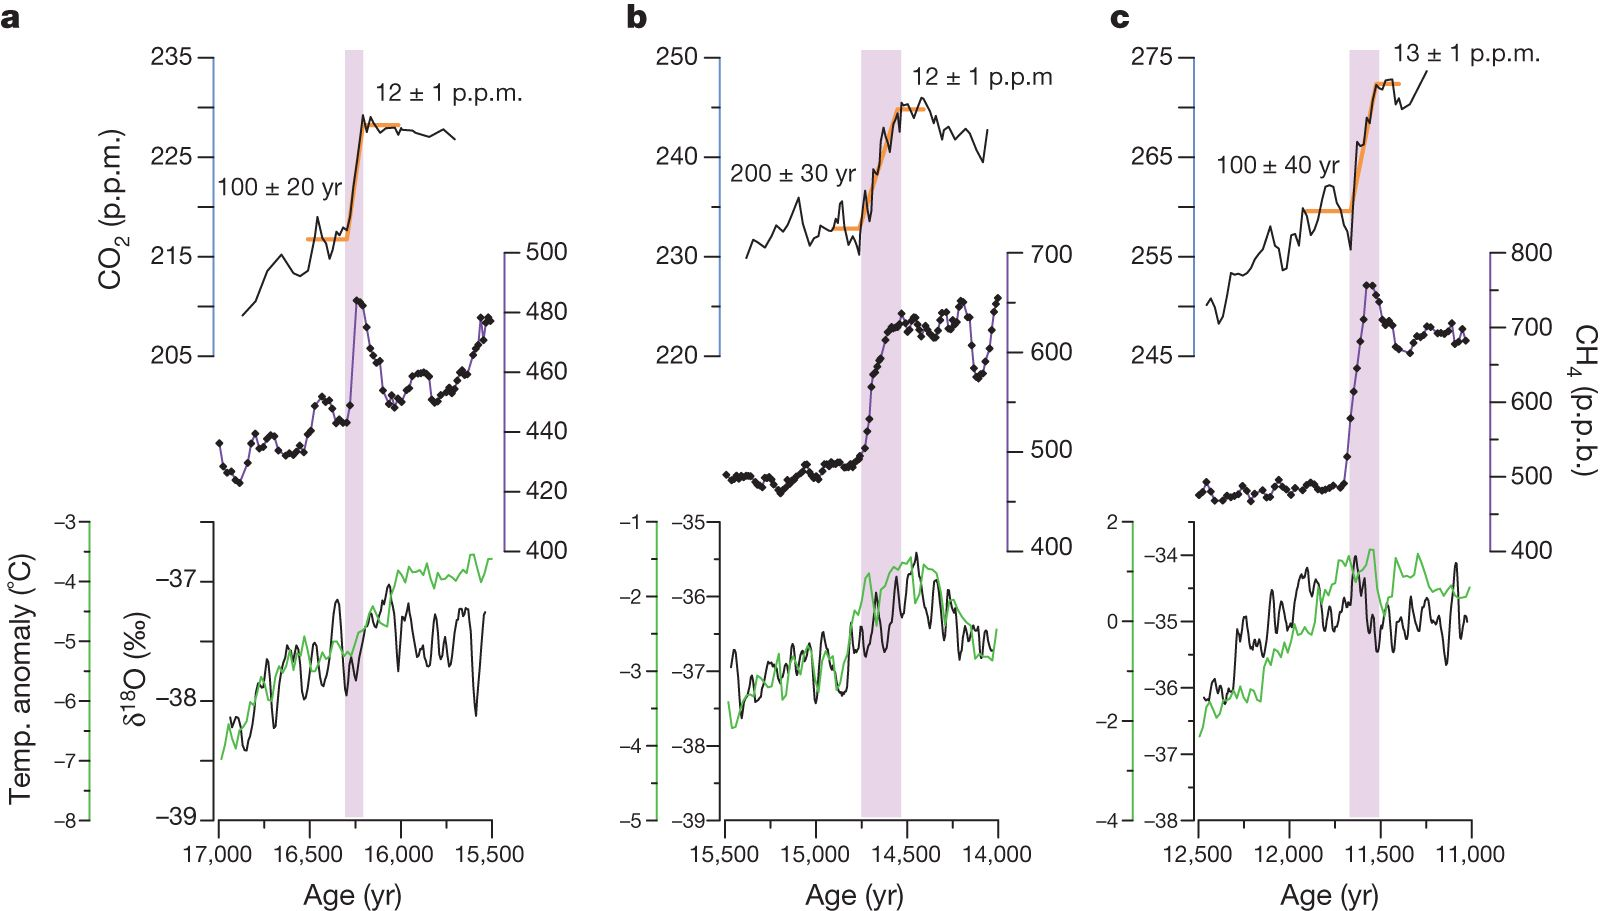
\includegraphics[width=.95\textwidth]{img/marcott2014.jpg}
	
	\smallskip\noindent\small Zmiany poziomu dwutlenku węgla pod koniec ostatniej epoki lodowej. Źródło: Marcott et al.~(2014).
\end{figure}

Na koniec wypada zauważyć, że współczesny wzrost temperatury i gazów cieplarnianych tylko powierzchownie przypomina sytuację z okresu preborealnego. Wzrost zawartości dwutlenku węgla, o którym pisze KNG, nastąpił w tempie 15 ppm na około 100 lat\footnote{Marcott S.~A., et al.~(2014): ,,Centennial--scale changes in the global carbon cycle during the last deglaciation'', \doi{10.1038/nature13799}.}; obecnie zwiększenie poziomu o 15 ppm zajmuje tylko 5--6 lat. Również tempo wzrostu średniej globalnej temperatury było wtedy niższe niż obecnie, i najsilniej zaznaczało się w rejonie północnego Atlantyku\footnote{Shakun J.~D., et al.~(2012):~,,Global warming preceded by increasing carbon dioxide concentrations during the last deglaciation'', \doi{10.1038/nature10915}.}.

Oczywiście, samo to że 11 tysiące lat temu nastąpiła zmiana klimatu z przyczyn naturalnych nijak nie podważa roli dwutlenku węgla w \emph{obecnym} ociepleniu.

\newpage

\subsection*{O modelowaniu klimatu}

\begin{quotation}
	\textbf{Modele klimatyczne}
	
	Wzrost temperatury globalnej w ciągu ostatnich 300 lat (Fig.~3, Fig.~5) jest faktem, któremu zaprzeczyć nie można. Dyskusyjne jednak jest nie tylko tempo tego wzrostu w porównaniu do podobnych wzrostów znanych z poprzednich okresów historycznych (patrz rozdział poprzedni), lecz przede wszystkim prognozy na przyszłość, które tworzy się w oparciu o modele klimatyczne. W zasadzie wszystkie modele (przygotowane przez mocne zespoły badawcze i publikowane w najlepszych czasopismach naukowych), przewidywały wzrost temperatury na Ziemi w latach 1975--2025. Średnia wzrostu dla wszystkich modeli wyniosła ok. 1{,}2\si{\celsius} (Fig.~6), przy czym wyniki znacząco różniły się między sobą. Co więcej, współczesne pomiary temperatury w środkowej troposferze dają wynik trzykrotnie niższy od wartości średniej, przewidywanej przez omawiane  modele (Fig.~6). Podobnie, modelowanie klimatu w holocenie (ostatnie 11{,}2 tys.~lat --- por. Fig.~5, linia zielona) rozmija się z obserwacjami przyrodniczymi (Liu et al.~2014). Przyczyny takiego stanu rzeczy są przedmiotem dyskusji (przyjęte parametry wyjściowe dla modelowania, techniki pomiarowe, algorytmy programów obliczeniowych), wykraczającej poza zakres niniejszego opracowania.
\end{quotation}

\begin{figure}
	\centering
	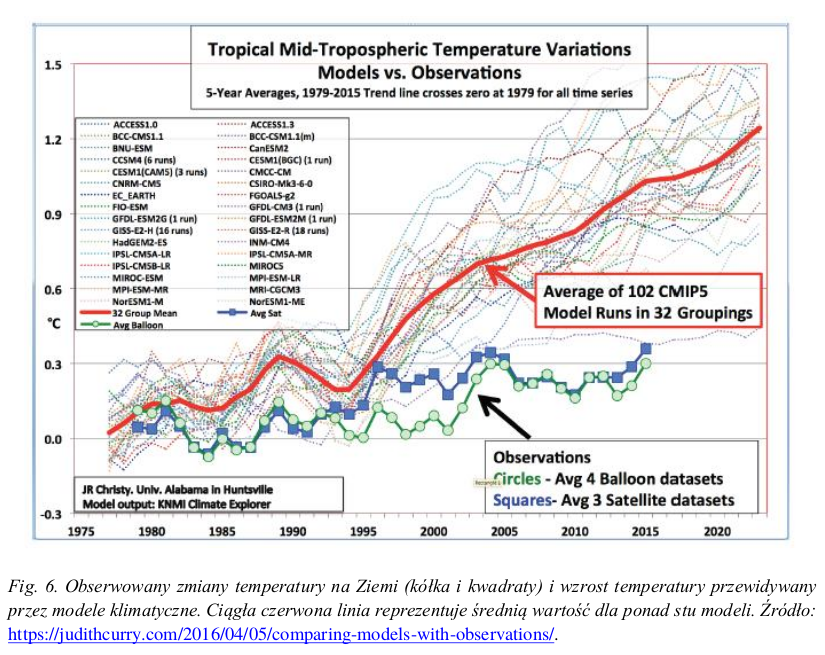
\includegraphics[width=.95\textwidth]{img/kng4.png}	
\end{figure}

Ponownie mogę tylko ubolewać nad tym, że geolodzy z KNG PAN korzystają z naprędce wygooglanych obrazków, i nie zadali sobie trudu by zajrzeć do źródeł naukowych, mimo że publikacji poświęconym pomiarom i modelowaniu temperatury troposfery są dosłownie dziesiątki, w tym niektóre zajmujące się szczegółowo wymienionymi wyżej zagadnieniami, jak rzekome trzykrotne zawyżenie tempa wzrostu temperatury\footnote{Santer B.~D., et al.~(2016):~,,Comparing Tropospheric Warming in Climate Models and Satellite Data'', \doi{10.1175/JCLI-D-16-0333.1}.}\footnote{Santer B.~D., et al.~(2017):~,,Causes of differences in model and satellite tropospheric warming rates'', \doi{10.1038/ngeo2973}.}\footnote{Thorne P.~W., et al.~(2011):~,,A quantification of uncertainties in historical tropical tropospheric temperature trends from radiosondes'', \doi{10.1029/2010JD015487}.}. Jest prawdą, że przewidywania przyszłych zmian klimatu w oparciu o symulacje modeli są obarczone niepewnościami; modele są z definicji niedoskonałym odzwierciedleniem rzeczywistości, i drobne różnice w odwzorowaniu procesów zachodzących w atmosferze i oceanach skutkują różnymi prognozami tempa i amplitudy zmian parametrów klimatycznych. Tym niemniej, wszystkie modele konsekwentnie przewidują znaczącą zmianę klimatu --- temperatury, opadów, zachmurzenia, cyrkulacji atmosferycznej --- jeśli będziemy kontynuować spalanie paliw kopalnych, a różnice pomiędzy prognozowanymi scenariuszami zawierają się pomiędzy wariantami ,,będzie źle'' i ,,będzie bardzo źle''.
		
Wykres, który znaleźli w internecie autorzy stanowiska KNG PAN, różnice te jednak zawyża, minimalizując jednocześnie niepewności związane z pomiarami temperatury troposfery: szeregi obserwacyjne zostały uśrednione, nie widać więc różnic pomiędy różnymi analizami pomiarów. W rzeczywistości obserwowane zmiany temperatury pozostają w obrębie wiązki symulacji przeprowadzonych w ramach projektu CMIP5 (choć w dolnym jej zakresie, co oznacza że średnio większość modeli zawyża nieco tempo zmian temperatury troposfery).

\begin{figure}
	\centering
	
	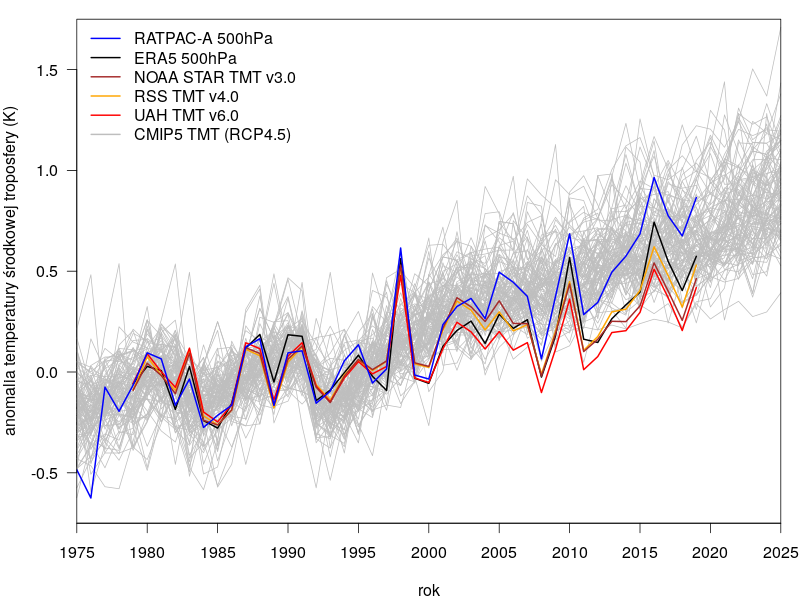
\includegraphics[width=.95\textwidth]{img/cmip5_tmt.png}
\end{figure}
		
Porównanie wyników modelowania zmian klimatu holocenu jest jeszcze bardziej skomplikowane. Cytowany przez KNG artykuł Liu i in.\footnote{Liu Z., et al.~(2014):~,,The Holocene temperature conundrum'', \doi{pnas.1407229111}.} wskazuje, że choć faktycznie źródłem rozbieżności symulowanych i rekonstruowanych trendów temperatury mogą być błędy modeli, a konkretnie zbyt słabe sprzężenia zwrotne związane z albedo lodu i śniegu, przynajmniej za część rozbieżności może też odpowiadać błędy rekonstrukcji paleoklimatycznych, wynikające z biasów sezonowych i przestrzennych\footnote{Baker J.~L., et al.~(2017): ,,Holocene warming in western continental Eurasia driven by glacial retreat and greenhouse forcing'', \doi{10.1038/ngeo2953}.}\footnote{Marsicek J., et al.~(2018):~,,Reconciling divergent trends and millennial variations in Holocene temperatures'', \doi{10.1038/nature25464}.}. Dodam jeszcze, że problem nie dotyczy \emph{tylko} rozbieżności pomiędzy modelami z jednej strony a rekonstrukcjami z drugiej, ale również pomiędzy rekonstrukcjami opartymi o różne typy proxy.
			
Niezależnie od przyczyny, wpływ niepewności związanych z przyczynami i przebiegiem zmian klimatu w holocenie mają niewielki wpływ na naszą ocenę przyczyn \emph{obecnego} globalnego ocieplenia. Jak wyjaśniałem w poprzednich częściach komentarza, wiedza dotycząca odległej przeszłości zawsze będzie obciążona większymi niepewnościami, więc nierozstrzygnięte jeszcze rozbieżności pomiędzy symulacjami a rekonstrukcjami nie są wystarczającym powodem, by odrzucać ustalenia oparte o \emph{współcześnie} przeprowadzane pomiary i~obserwacje.

\newpage

\subsection*{O wyciąganiu wniosków}
			
\begin{quotation}
	\textbf{Podsumowanie i wnioski praktyczne}	

	Dane geologiczne, analizowane w różnych skalach czasowych, nie potwierdzają prostej uniwersalnej zależności przyczynowo-skutkowej między wzrostem poziomu CO$_2$ w atmosferze a wzrostem temperatury, sugerując większą złożoność zjawiska zmienności temperatury naszej planety. Z drugiej strony nie wykluczają takiej zależności w konkretnych przypadkach, a w szczególności zjawiska sprzężenia zwrotnego, czyli wzmacniania naturalnego trendu wzrostu temperatury przez wywołane tym wzrostem, ale także antropogeniczne, podnoszenie się poziomu CO$_2$ w atmosferze. Wynika stąd wniosek, że nawet jeśli obserwowany obecnie wzrost temperatury jest zjawiskiem naturalnym, to antropogeniczny CO$_2$ może ten trend wzmocnić. Jeśli zatem wzrost temperatury uznajemy za zjawisko niepożądane, to należy próbować go minimalizować. Głównym dostępnym ludzkości działaniem w tym kierunku jest ograniczenie spalania węgla i węglowodorów, gdyż emitujemy rocznie ok.~$3{,}7\times10^{10}$ ton CO$_2$/rok (Le Quéré et al., 2018), tj. o dwa rzędy wielkości więcej niż obecnie wszystkie wulkany na Ziemi razem wzięte ($2\times10^{8}$ ton rocznie, wg US Geological Survey).
\end{quotation}

Dane geologiczne nie potwierdzają prostej uniwersalnej zależności przyczynowo-skutkowej między wzrostem poziomu CO$_2$ w atmosferze a wzrostem temperatury, bo temperatura Ziemi nie zależy tylko od poziomu CO$_2$ w atmosferze. Istnieją też inne czynniki, z których niektóre mają znaczenie tylko w geologicznej skali czasu, jak konfiguracja kontynentów albo ewolucja Słońca na diagramie Hertzsprunga--Russella. Tym niemniej, po uwzględnieniu tych czynników okazuje się, że \emph{obecne} ocieplenie planety nie jest ,,naturalnym trendem wzrostu temperatury'', i~że antropogeniczny dwutlenek węgla i inne gazy cieplarniane z nawiązką wystarczają do wytłumaczenia tego zjawiska.
			
\begin{quotation}
Spalając węgiel i węglowodory kopalne odwracamy bieg naturalnych procesów geologicznych. Ostatnie dwa miliardy lat, a w szczególności ostatnie pół miliarda lat, to okres naturalnej sekwestracji dwutlenku węgla (fotosynteza) z atmosfery do skorupy ziemskiej poprzez grzebanie materii organicznej w osadach i jej przekształcanie w złoża węgla oraz węglowodorów stałych, płynnych i gazowych (metan). Równolegle CO$_2$ był sekwestrowany dzięki wietrzeniu chemicznemu w postaci skał węglanowych. Węgiel odkładał się w skorupie powoli i dość systematycznie, czego efektem był blisko dwudziestokrotny spadek koncentracji CO$_2$ w atmosferze --- od ok. 7000 ppm ($\pm40\%$) w kambrze (Fig.~1) do poziomu ok.~300 ppm w roku 1950. Z punktu widzenia ewolucji atmosfery ziemskiej dziś dwutlenku węgla prawie nie ma. Tak niski poziom koncentracji CO$_2$ w atmosferze mógł być --- podobnie jak w karbonie (Fig.~1) --- istotną przyczyną globalnego zlodowacenia, które zaczęło się ok.~33 mln lat temu powstawaniem pokryw lodowych na Antarktydzie i nasilało się aż do zamarznięcia Oceanu Arktycznego ok.~2 mln lat temu. Zgodnie z prawem Henry'ego, coraz zimniejszy ocean światowy pochłaniał coraz więcej CO$_2$, napędzając schładzanie powierzchni Ziemi poprzez zmniejszanie efektu cieplarnianego (w myśl tego samego prawa, ogrzany ocean odda do atmosfery nadmiarowy CO$_2$). W efekcie, mamy dziś największe zlodowacenie globalne w ciągu ostatniego pół miliarda lat. Przyszliśmy na świat w tym wyjątkowym czasie i, chcemy czy nie, jesteśmy dziećmi globalnego chłodu. Istnieje ryzyko, że wraz z jego odejściem, odejdziemy i my. Wydaje się zatem roztropne podtrzymanie obecnego stanu geosystemu jak najdłużej będzie to możliwe.
\end{quotation}

Ten fragment jest o tyle interesujący, że w miarę poprawnie (pomijając kilka nieścisłości, które prostowałem już wcześniej) opisuje cywilizację przemysłową jako czynnik odwracający, poprzez utlenianie paliw kopalnych, trwające miliony lat naturalne procesy geologiczne, co oczywiście kontrastuje z próbami minimalizacji wpływu człowieka na klimat, którą widać w poprzedzających akapitach.
			
\begin{quotation}
	Z pragmatycznego punktu widzenia, najbardziej skuteczne są/będą te działania, które wykorzystują procesy pochłaniania CO$_2$ i usuwania go z atmosfery w takiej ilości, w jakiej jest emitowany do atmosfery wskutek działalności człowieka. Z czystej przezorności, należy jednak rozważyć scenariusze najgorsze z możliwych i zacząć działania adaptacyjne, niezależnie od tego czy scenariusze te są, czy nie są prawdziwe.
\end{quotation}			

Zadziwiające, że KNG PAN nie mówi tutaj wprost o konieczności redukcji emisji dwutlenku węgla, mimo że bez tego nie da się wdrożyć technologii wychwytywania i składowania CO$_2$ na skalę wymaganą do zrównoważenia tychże emisji.
			
\begin{quotation}
	Spory naukowe dotyczące roli CO$_2$ w procesie zmian klimatu, często uwarunkowane konfliktami grupowymi lub personalnymi, powinny iść torem przyjętym w dyskursie naukowym, a nie odbywać się na forum publicznym, gdyż rozbieżne oceny powodują zamęt pojęciowy, chaos informacyjny, a nawet panikę, szczególnie wśród młodzieży.
\end{quotation}
			
Święte słowa, ale z jakiegoś powodu członkowie KNG się do własnej rekomendacji nie stosują. Dlaczego nie prowadzą sporu naukowego dotyczącego roli CO$_2$ torem przyjętym w dyskursie naukowym? Gdzie ich badania na ten temat, wystąpienia konferencyjne, recenzowane publikacje? Dlaczego wypowiadają się przede wszystkim na forum publicznym, w mediach masowych\footnote{\href{https://wnet.fm/2019/12/11/profesor-marks-o-klamstwie-klimatycznym-wymieraniu-gatunkow-braku-wody-zmianach-w-przyrodzie-i-produkcji-co2/}{,,Profesor Marks o kłamstwie klimatycznym\ldots''}} i prasie\footnote{\url{https://www.niedziela.pl/artykul/97579/nd/Klimat-wokol-klimatu}}, i drugi już raz wprowadzają zamęt pojęciowy i~chaos informacyjny publikując stanowisko niezgodne z ustaleniami nauki?
			
,,Panikująca'' młodzież jest już bardziej ogarnięta niż trzydziestu kilku profesorów geologii. Przynajmniej wie, jak cytować raporty IPCC\footnote{\url{https://www.rev.com/blog/transcripts/greta-thunberg-un-climate-change-conference-speech-transcript}}.
			
\begin{quotation}
	Skomplikowane procesy, które rządzą klimatem, wymagają prowadzenia interdyscyplinarnych badań przez różne grupy o różnych specjalnościach, nie tylko w ramach IPCC, z pewnością także i w Polsce. Powinny to być badania cyklicznych fluktuacji klimatycznych w przeszłości Ziemi i ich uwarunkowań odczytywanych z zapisu kopalnego, monitorowanie poznanych dotąd czynników sprawczych, modelowanie ich udziału w przekształceniach klimatu i weryfikowanie sporządzanych modeli w odniesieniu do zdarzeń przeszłych dla oceny ich wiarygodności w prognozowaniu zdarzeń przyszłych.
\end{quotation}			

Takie badania się oczywiście od dawna prowadzi, i biorą w nich udział również polscy geolodzy\footnote{Np.~Niezgodzki I., et al.~(2019):~,,Was the Arctic Ocean ice free during the latest Cretaceous? The role of CO$_2$ and gateway configurations'', \doi{10.1016/j.gloplacha.2019.03.011}.}.
			
Niestety, interdyscyplinarne badania prowadzone przez różne grupy o różnych specjalnościach nie przyniosą żadnego pożytku, jeśli ich wyniki są ignorowane, tak jak autorzy stanowiska KNG PAN ignorują ustalenia nauki w~temacie przyczyn obecnego globalnego ocieplenia, a~także zmian klimatu w~odległej przeszłości Ziemi.
\end{document}